\chapter{Deliverables}
    \label{chap:deliverables}
    This chapter will present the deliverables produced during the project in the order of the stages defined in the software development model.  Section~\ref{sec:deliverables_requirements} will cover the requirements analysis, Section~\ref{sec:deliverables_design} will contain the design documentation, Section~\ref{sec:deliverables_implementation} will discuss the implementation, and finally, Section~\ref{sec:deliverables_testing} will contain the testing documentation.
    
    \section{Description of project}
        \label{sec:deliverables_description}
        This project produces an application available on the iOS platform only, with the potential to be expanded to other platforms such as iPadOS, WatchOS and Android; however, those platforms remain outside of this projects scope.  The application is built using the Swift programming language, and Firebase handles the interaction between the application and the Google servers.  The UI for the application is built using SwiftUI and UIKit.
        
    \section{Requirements Analysis}
        \label{sec:deliverables_requirements}
        The project requirements were based partly on what is seen as the basic features expected in a productivity and time-management application and partly on the results of the questionnaire that was sent to prospective users (Appendix~\ref{app::questionnaire}). This questionnaire collected data on the current employment status of the potential user and what feature would make them want to download and use a productivity application.  The questionnaire also asked the prospective users their thoughts on a task suggestion feature and whether they would utilise such a feature and why.
        
        Following this, a list of requirements was generated at the start of the project; however, it was expected that these requirements could change based on the obstacles reached during development.  Therefore, the revised set of requirements, split into functional and non-functional, has been defined and can be found in Table~\ref{app::requirements_table}.
        
        Compared to the requirements defined at the start of the project, some requirements have been removed, and some requirements were defined as "time-permitting"; these were not completed.  The removed requirements included seeing a friend's recent activity within the application. This was removed because the infrastructure needed to implement this requirement was not available.  The requirements also defined the use of a tutorial when the user was first to use the application, however, this requirement was also removed due to the application being self-explanatory.  The non-compulsory requirements included adding items using Siri (the virtual assistant available on Apple devices) and being able to add and complete items displayed in a 'Widget', which was a new feature provided by Apple when iOS 14 was released in 2020.  Due to time constraints, neither of these requirements were included.
        
    \section{Design}
        \label{sec:deliverables_design}
        In the sections below, the designs produced for the project will be presented and discussed.  The designs will include the UI design (Section~\ref{subsec:UI_design}), Data flow design (Section~\ref{subsec:DFD}), entity relationship design (Section~\ref{subsec:E-R_diagram}) as well as testing design (Section~\ref{subsec:test_design}).  Each section will include a short reflection, including whether the designs were met in the implementation and whether any changes were made.
        
        \subsection{User Interface Design}
        \label{subsec:UI_design}
        For the UI design, wireframe designs were first created to get an idea of how the application should generally look without deciding on colours and fonts.  These wireframes were created using Balsamiq Mockups 3 and can be viewed in Section~\ref{app::mockups} of the appendix.  The application is designed to have a minimalist type theme, so an attempt was made to ensure the UI was self-explanatory and straightforward in terms of features.  There is a navigation bar placed at the bottom of the application, which remains consistent throughout all the views to ensure the application's navigation is easy. Every screen is only one tap away.
        
        In Section~\ref{app:colour} of the appendix, the coloured designs based on the wireframe mock-ups can be found.  At this point in the design process, a colour scheme had been chosen (Figure~\ref{fig:colour_scheme}) and the font scheme and the icons provider.  The font scheme chosen was the Montserrat family, and the icons would be sourced from the site icons8 as they had free icons that could be used in the application.
        
        \begin{figure}[H]

	\centering
	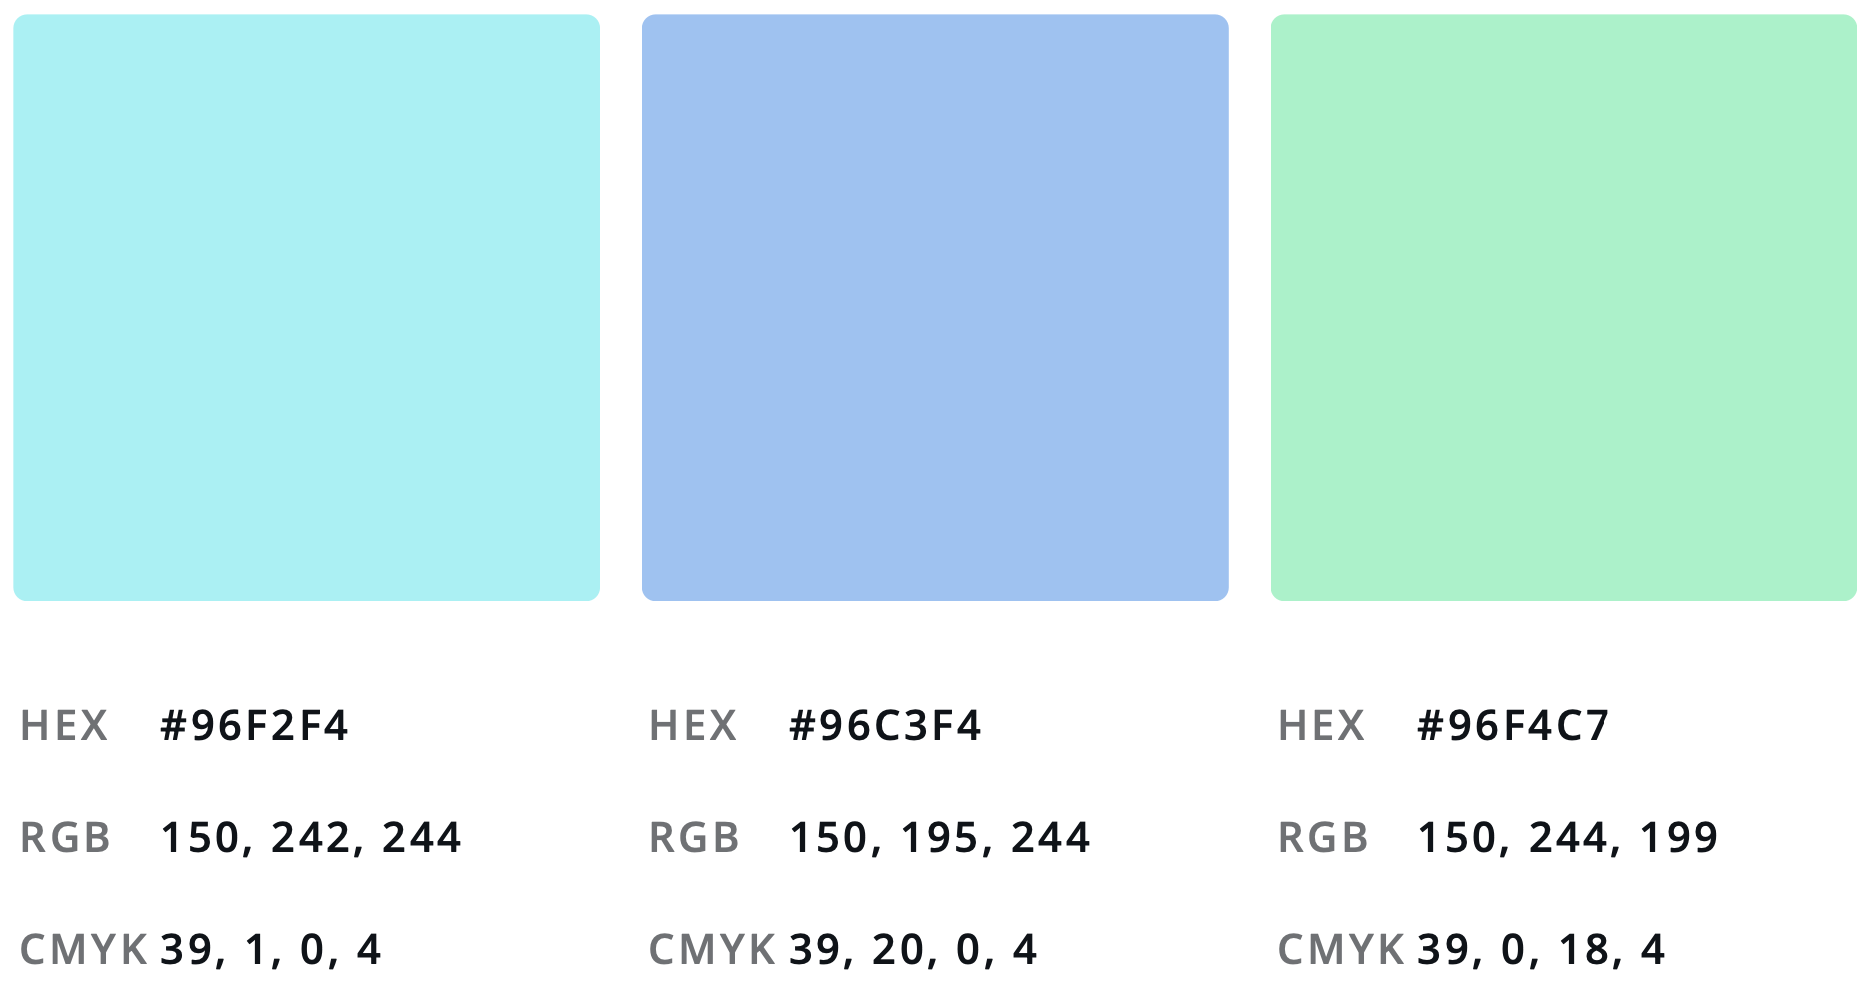
\includegraphics[width=4cm]{./graphics/design/Colours.png}
	\caption{The colour scheme used in the application.}
	\label{fig:colour_scheme}
	
\end{figure}
        
        Overall, the application was mainly able to imitate the designs produced. However, some changes did need to be made.  An attempt was made to use the Montserrat font family in the application. However, XCode did not seem to support this, and the application would render with the default system font usually provided with iOS applications.  The streak statistics initially shown in the wire-frames were not continued into the coloured design or the application because this feature was unable to be provided due to limitations with the SwiftUI framework. The design also showed suggestions as events in the calendar view. However, this was not possible during implementation due to limitations with the third-party library used, so suggestions are now only made in the agenda view.  The designs contained a recent activity screen that could be navigated to from the 'friends' screen.  The recent activity view was still a feature in the final application but does not show a friend's recent activity.  It became apparent later in the implementation phase that this feature was not accounted for when designing the database. So it was not possible to add it into the application without significantly affecting the completion deadline, however, in future this feature could be added to the application.
        
        \subsection{Data Flow Diagrams}
        \label{subsec:DFD}
        Section~\ref{app:dfd} of the appendix shows the data flow diagrams generated during the project's design phase.  These diagrams show the flow of data between the user, the application and the database.  
        
        Figure~\ref{fig:signin_signup_dfd} shows the data flow for the sign in and sign up views.  The user inputs their login data into either the sign in or sign up view.  The sign in view will authenticate the user with the database, and the database will either return an authentication error or successfully authenticate the user.  The sign-up view will add the user to the database, and the database will either return with an error saying the user already exists or will successfully add the new user.
        
        Figure~\ref{fig:dashboard_allitems_dfd} shows the data flow between the dashboard and the all items view. The user will input item data into the add item view.  They then have the option to save the item to the database or cancel the action.  Cancelling the action will take the user back to the dashboard or the all items view, depending on which view the user accessed the add item view from. If the user saves the item, it will be saved to the database, and then the application will automatically navigate back to the dashboard or the all items view.  Both the dashboard and the all items view will then request a list of all items saved to the users' account from the database, and this list will then be displayed.
        
        Figure~\ref{fig:focus_dfd} shows the data flow for the focus view.  The user will input timer data when amending the focus timer settings, and these settings will then be passed to the main focus view.  These settings will be saved locally on the device.
        
        Figure~\ref{fig:friends_dfd} shows the data flow for the 'friends' view.  The user will input the user email they wish to add into the add friend view, and this will be sent to the database to search to see if the email exists.  If the email exists, the relevant data from that user account will be sent to the main 'friends' view.  When the 'friends' view is brought to the foreground of the application, it will request a list of all the user accounts the current user is associated with, and these user accounts will be passed to the view by the database.
        
        The data flow in these diagrams seemed to remain accurate during the implementation and would look very similar if they were reproduced again with the application already built.  However, they may have been more helpful if they were slightly more accurate; the database could have been specified more specifically. The application communicates with a user database that contains email and passwords only, and then another database containing item data associated with a user ID.
        
        \subsection{Entity-Relationship Diagrams}
        \label{subsec:E-R_diagram}
        Section~\ref{app:er} of the appendix shows the entity-relationship diagram produced during the design phase of the project.  The diagram shows the different objects stored in the database and the relation they have to each other and the user object.
        
        The user object is shown as having an email, password, and username, with the email and username making the primary key.  The event object is shown as having an ID, name, date, time and labels, with the ID being the primary key.  The reminders object is shown as having the same attributes as the event object.  The task object is shown as having the same as the reminder and event object, but with a habit element added.  One user can create one or more of an event, reminder or task. One reminder can have one event.  One reminder can have one task.
        
        Due to the ambiguity of how the database would work at the beginning of the project, this entity relationship diagram is no longer an accurate representation of how the various entities within the application are linked.  There are still events, reminders and tasks, and these can be generated as separate objects. However, all of them are derived from the same object named 'Item'.  Also, the user object was created without a username and has a unique ID generated by Firebase, which cannot be seen in the diagram.  The elements connected to the event, reminder and task entities are accurate.  An Item object contains all of these elements, so that is the only part of the diagram that remained consistent with the application.
        
        \subsection{Test Design}
        \label{subsec:test_design}
        The testing methods to be used during the project included UI testing, user testing and ad-hoc testing.
        
        For UI testing, it was decided that a "record and replay" approach would be taken as this was a feature already available in XCode and could mostly be automated.  This approach involves recording various interactions with the UI and then the IDE repeating these interactions during a test.  If the desired result is achieved, the test passes.  As a result, the "record and replay" tests were not included in the test design as it was unclear in many cases how exactly the application would behave in response to UI interaction.
        
        Ad-hoc testing involves using the application without any reference to a specific test case or plan\cite{software_testing}. This method was chosen because it was decided this was the quickest way to test the application as it does not require a test suite, therefore making the testing design time frame minimal. Testing could be mostly completed during the implementation phase.
        \vspace{\baselineskip}
        
    \section{Implementation}
    \label{sec:deliverables_implementation}
        In this section, the implementation of the application will be discussed. This will include talking through how the front-end was developed and an examination of the back-end, with code snippets and screenshots of the UI results available in the appendix.
        
        \subsection{Splash/Sign Up/Sign In}
        \subsubsection{Front-end}
        The splash screen was the only view in the entire application that used a storyboard file to create the view.  Storyboards are a feature native to UIKit but have been replaced with SwiftUI files with the introduction of the SwiftUI framework.  A storyboard was used for the splash screen because this was the default set up when a new project was created, and as the splash screen UI only contains a single label, it was felt that there was no need to change this.
        
        The UI for the sign-up and sign in views is very similar, with only the buttons' destination and the labels being slightly different. The sign-up view contains three text fields that allow the user to input a username, email and password. They can then click on the 'create account' button, which will validate their credentials and show the dashboard view (Figure~\ref{fig:splash_signup_signin_app}). If the user wishes to sign in with Facebook, they do not need to type in any credentials on the sign-up screen; they can tap the 'sign up with facebook' button, which will open a view taking them through the usual Facebook login. Images of the Facebook login process can be found at ~\ref{app:facebook_login_frontend} of the appendix.  After this is successful, the application will then navigate to the dashboard view. If the user taps on the 'sign in' button from the sign-up view, they will be taken to the sign-in view, where they can log in using their email and password or the Facebook login. Once again, successfully logging in will take them to the dashboard view.
        
        \begin{figure}[H]
    \centering
    \begin{subfigure}[b]{0.3\textwidth}
        \centering
        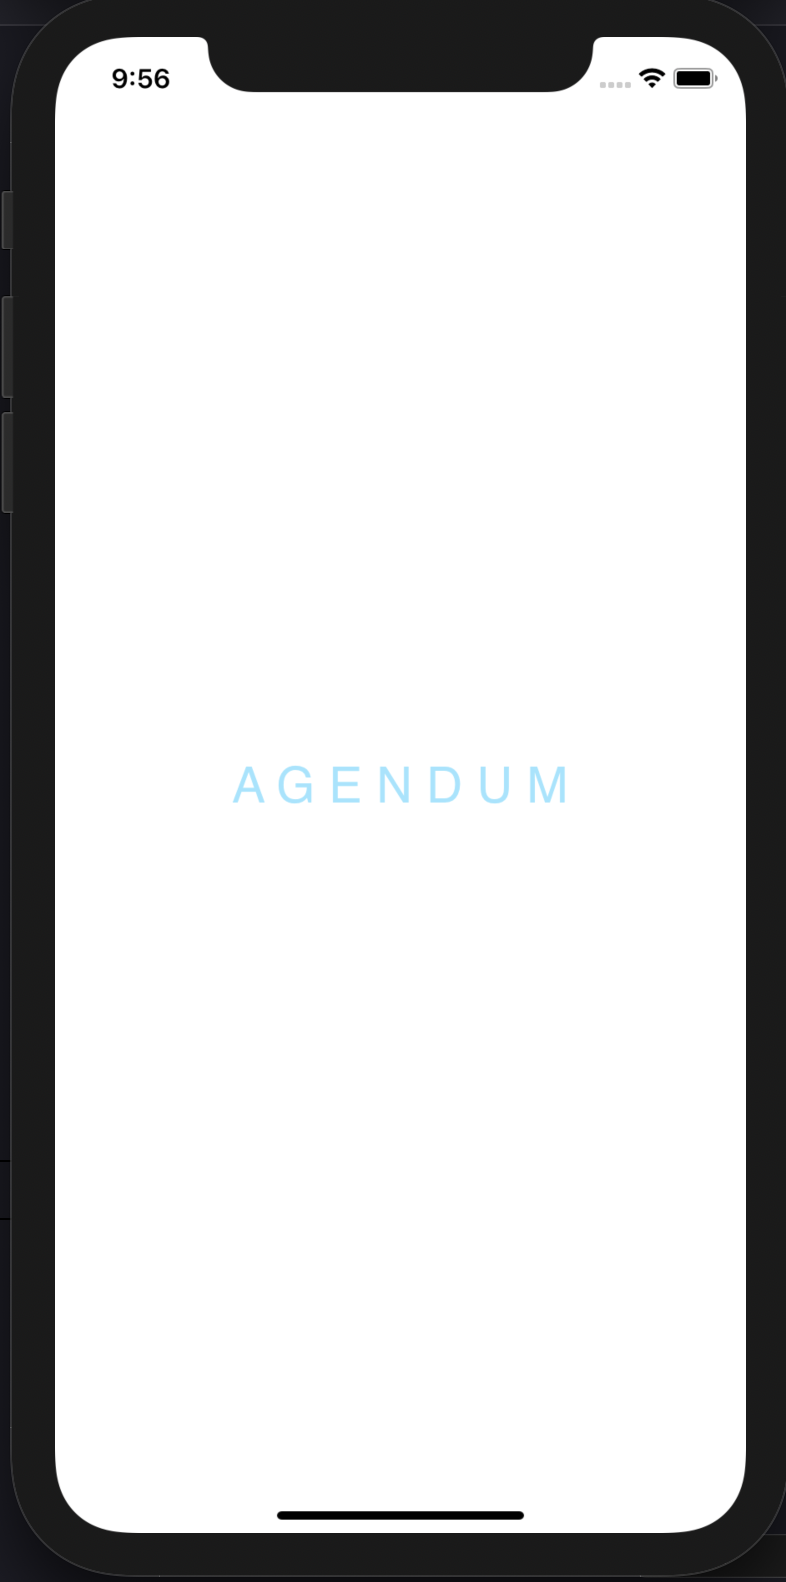
\includegraphics[width=\textwidth]{./graphics/Implementation/Splash_Sign_Up_Sign_In/splash.png}
        \caption{Splash Screen.}
        \label{fig:splash_app}
    \end{subfigure}
    \hfill
    \begin{subfigure}[b]{0.3\textwidth}
        \centering
        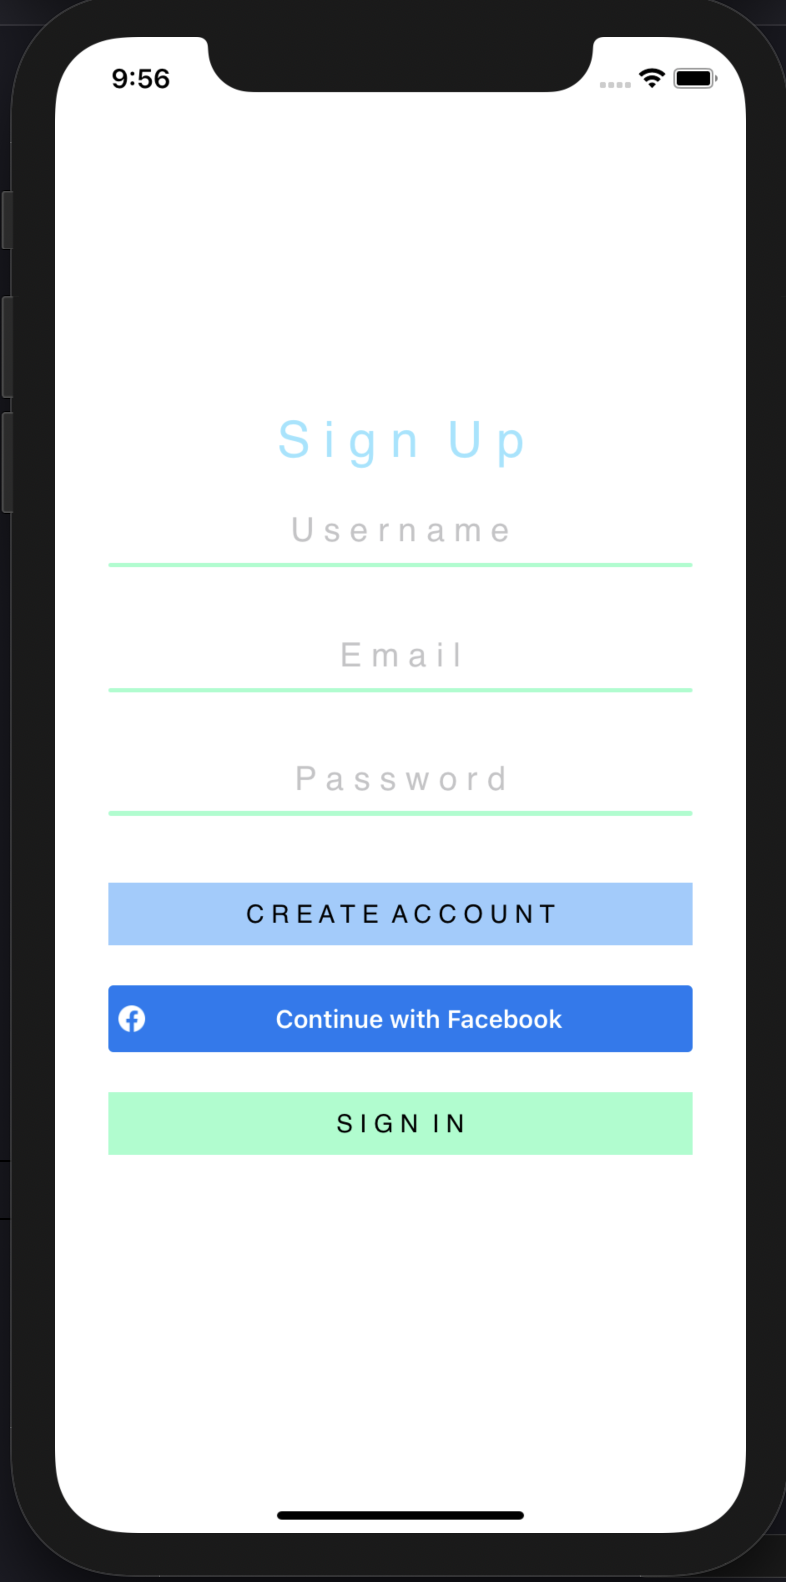
\includegraphics[width=\textwidth]{./graphics/Implementation/Splash_Sign_Up_Sign_In/signup.png}
        \caption{Sign Up.}
        \label{fig:sign_up_app}
    \end{subfigure}
    \hfill
    \begin{subfigure}[b]{0.3\textwidth}
        \centering
        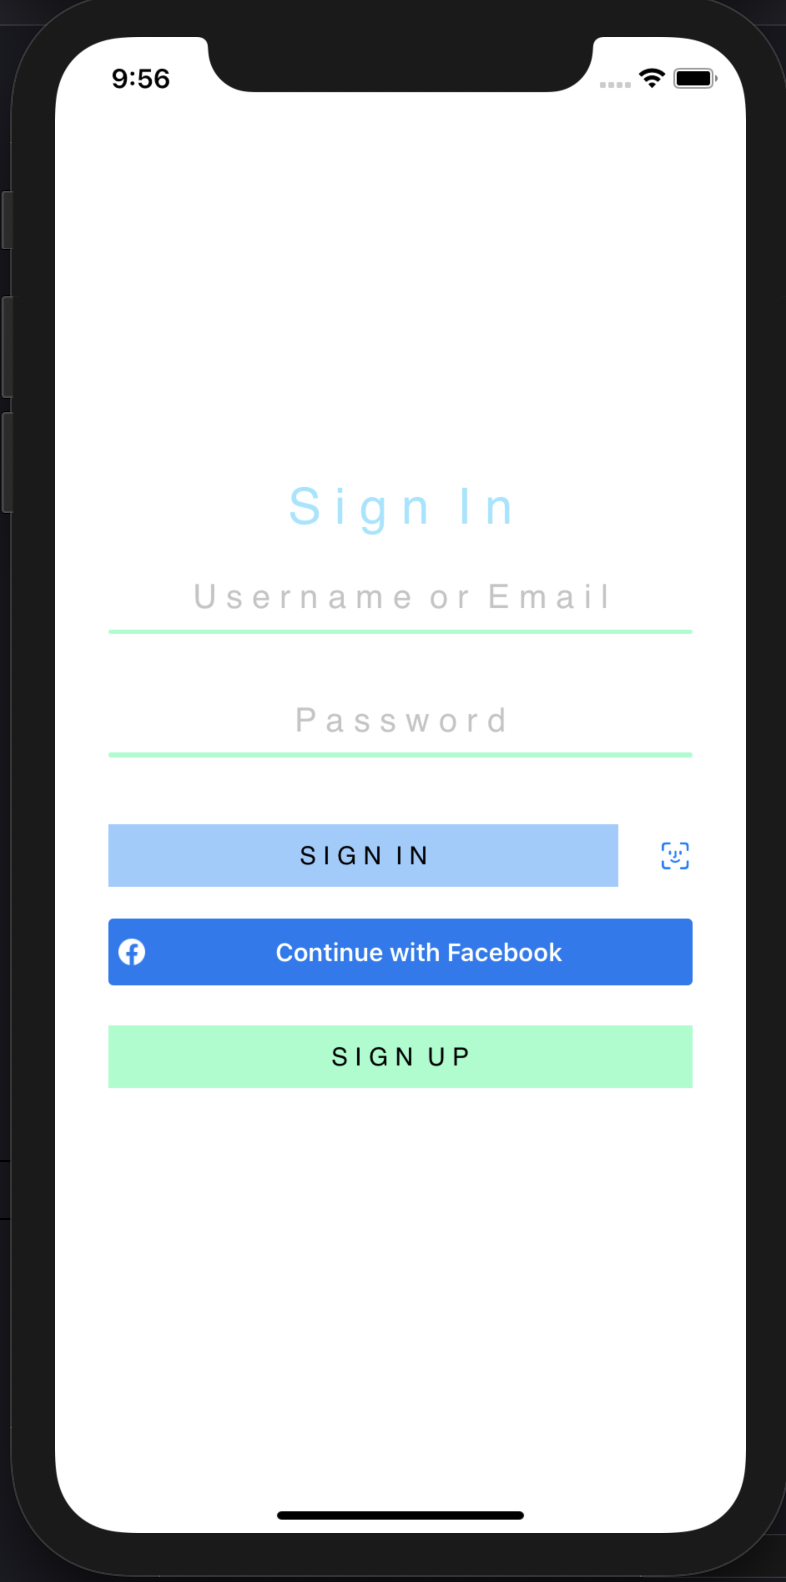
\includegraphics[width=\textwidth]{./graphics/Implementation/Splash_Sign_Up_Sign_In/signin.png}
        \caption{Sign In.}
        \label{fig:sign_in_app}
    \end{subfigure}
    
    \caption{Splash, sign up and sign in views shown in the application.}
    \label{fig:splash_signup_signin_app}
\end{figure}
        
        \subsubsection{Back-end}
        To officially register or log in a user, the application uses a class that communicates with the Firebase database using the Firebase API, installed using Cocoapods.  The code snippets for this class can be found in ~\ref{app:splash_signup_signin_backend} of the appendix.  The listen function is used to monitor authentication changes in the database.  If a change is detected, then the current logged in user is retrieved from Firebase, and the data returned is used to populate the User object within the application. The addUser function communicates with the Firestore database, populates the database with the user ID and adds an empty progress value.  This allows a user to add another user, as it is not possible to directly access the authenticated user database in Firebase for security reasons.  The addUsername function makes a call to the Firebase API to update a user profile and adds a username to that profile; however, during the development of the application, the use of usernames became obsolete as the user email is used to find other users and to primarily sign users in. The signIn and fbSignUp functions both make a call to the signIn function provided in the Firebase API but with slightly different parameters.  The regular sign-in uses email and password, but if Facebook sign-in is used, an AuthCredential object is passed as a parameter.  Finally, signUp makes a call to the createUser function provided in the Firebase API, and this uses email and password as parameters.  After this call is successful, the User object in the application is updated. The user password is stored in Apple Keychain to be used if bio-metrics is enabled in the application settings.
        
        When the user creates an account on the application, the storeGenericPasswordFor function will be called from the KeychainWrapper class.  This function simply stores the users' password in the relevant keychain directory and is secured by the iOS system.  When the user then attempts to sign in to the application with biometric authentication, the getGenericPasswordFor function will be called so that a password can be passed as a parameter to the signIn function contained in the FirebaseSession class.
        
        \subsection{Dashboard}
        \subsubsection{Front-end}
        The dashboard view contains many sub-views that handle the applications' primary purpose, which is to create and complete tasks.  All views in the dashboard will have to time frame at the top, the progress bar, and whether the view is in agenda or calendar mode.  The titles are custom elements made up of a Text object and a Horizontal Line object.  The progress bar is a Progress View object.
    
        The dashboard's default view is the agenda today view, which will show the items that need to be completed today in list form.  The items are split into events, reminders, tasks and suggestions, and are placed into these categories depending on the settings chosen when creating the item.  Each item is created from a Simple Task View, which is obtained from the CareKit module.  The view also contains an add button in the bottom right-hand corner, which will navigate the application to the add item view when tapped.  From this view, the user has a choice to swipe left on 'today' to switch to 'this week' or 'this month', or to swipe left on 'agenda' to switch to the calendar view for the corresponding time frame.  The swiping gesture is made possible because of the SwiftUIPager library, which allows the titles to be encapsulated in a Pager object.
        
        \begin{figure}[H]
    \centering
    \begin{subfigure}[b]{0.3\textwidth}
        \centering
        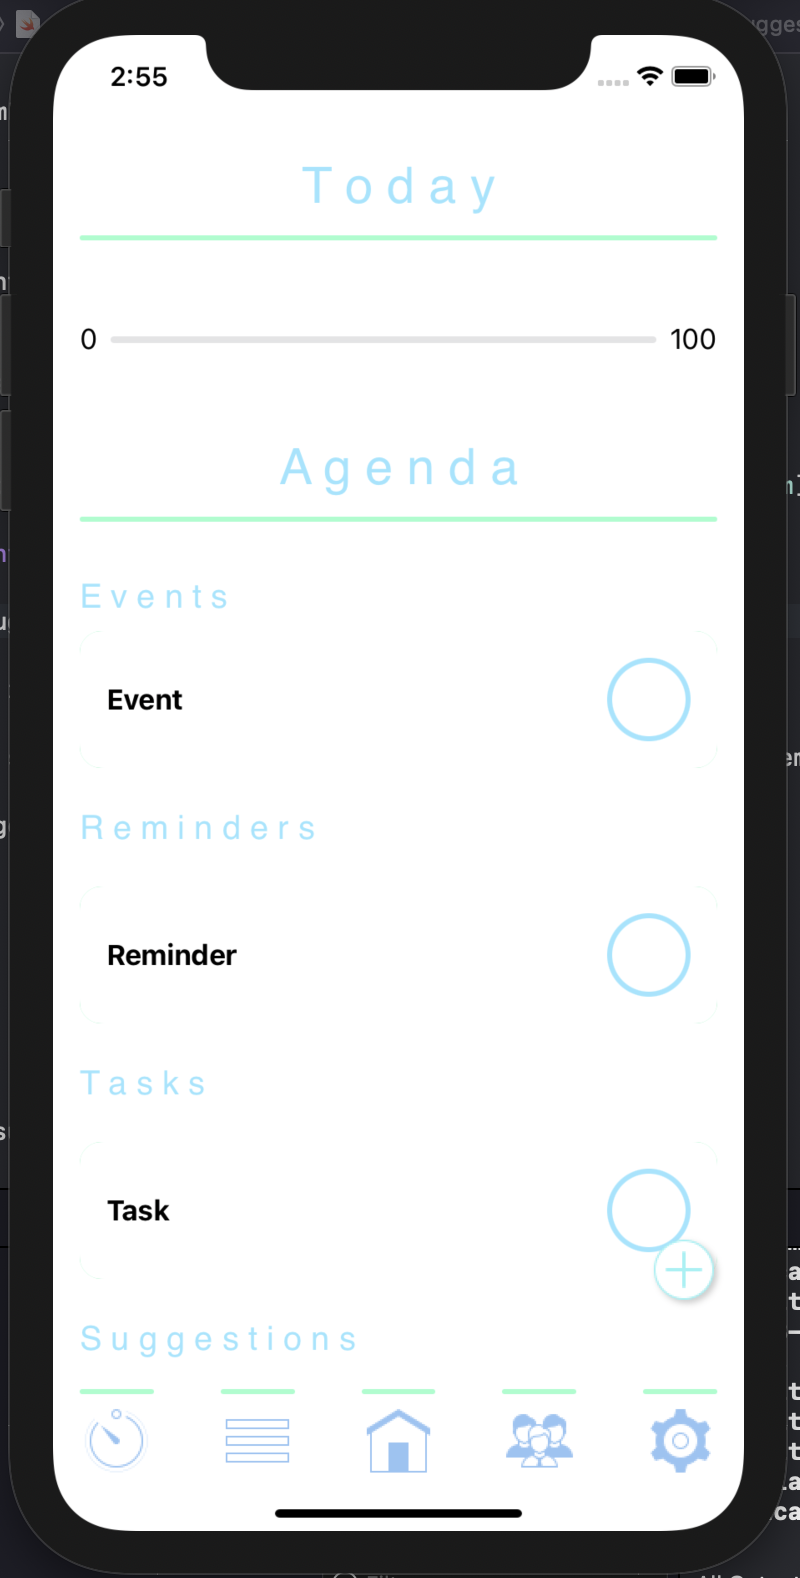
\includegraphics[width=\textwidth]{./graphics/Implementation/Dashboard/agenda today populated.png}
        \caption{Agenda Today.}
        \label{fig:agenda_today_app}
    \end{subfigure}
    \hfill
    \begin{subfigure}[b]{0.3\textwidth}
        \centering
        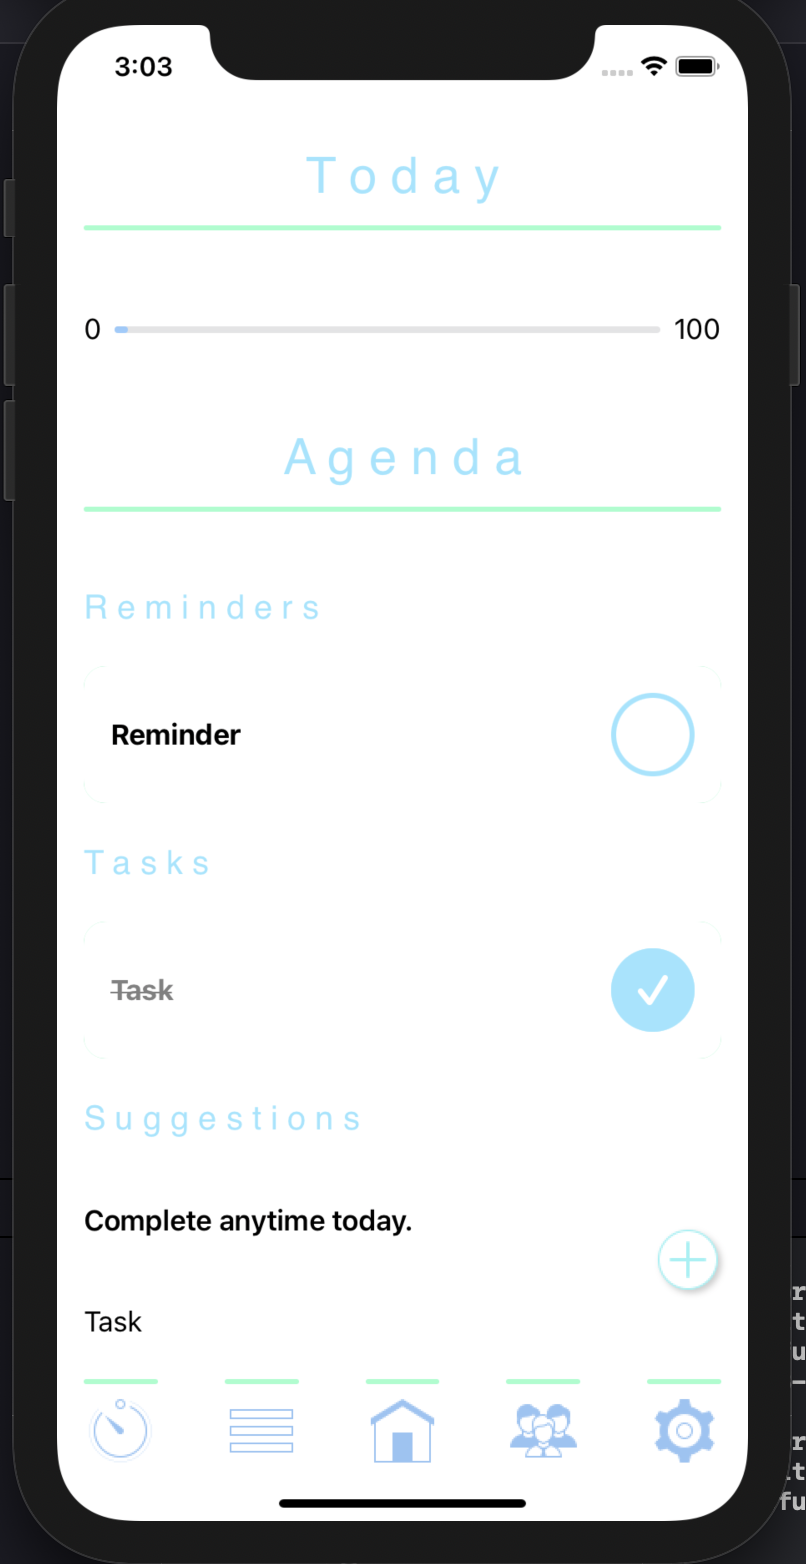
\includegraphics[width=\textwidth]{./graphics/Implementation/Dashboard/agenda today completed task.png}
        \caption{Task completed.}
        \label{fig:agenda_today_complete_app}
    \end{subfigure}
    \hfill
    \begin{subfigure}[b]{0.3\textwidth}
        \centering
        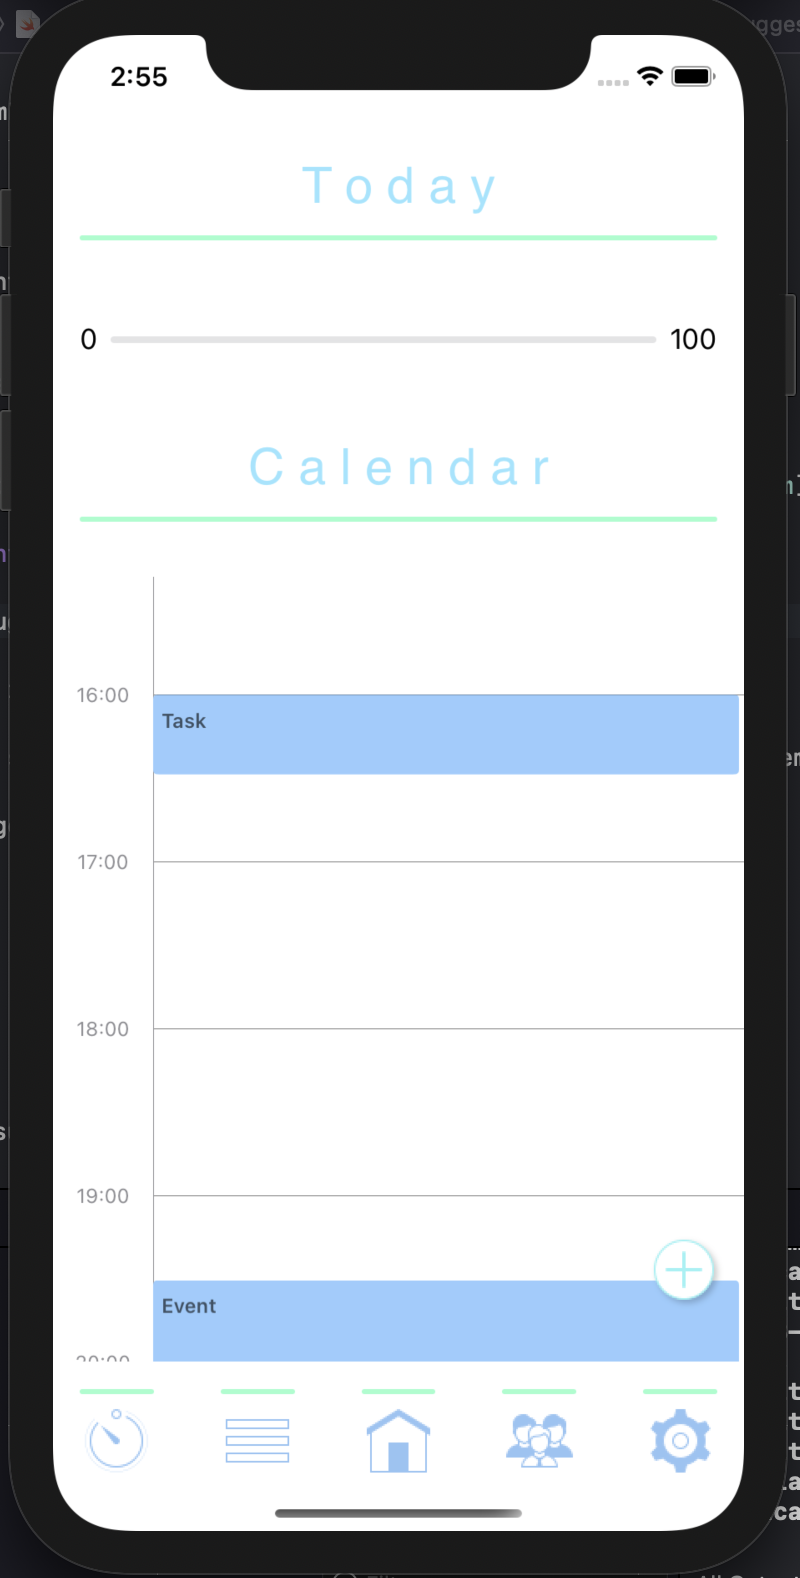
\includegraphics[width=\textwidth]{./graphics/Implementation/Dashboard/calendar today populated.png}
        \caption{Sign In.}
        \label{fig:calendar_today_app}
    \end{subfigure}
    
    \caption{The agenda and calendar today views.}
    \label{fig:agenda_calendar_today_app}
\end{figure}
        
        The agenda view for the other time frames is identical to the 'today' view. However, the calendar view for each time frame is slightly different.  The calendar for the 'today' time frame will show an hour-by-hour calendar for one day only.  This weeks' calendar will show an hour-by-hour calendar, but the user can choose from any day available during the week.  Finally, the calendar for this month shows a block for each day of the month, with a small dot indicator to show if there is an item during that day.  When the user taps on the day, a list of the items due will be shown below the calendar.
        
        When a user taps on a task in any of the calendar views, a view will appear on the screen with all the available details attached to that item and an option to edit the item.  If the user taps the edit button, they will be taken to the add item view. However, each element will already be populated with the item details, which can then be changed and saved.
        
        \begin{figure}[H]
    \centering
    \begin{subfigure}[b]{0.3\textwidth}
        \centering
        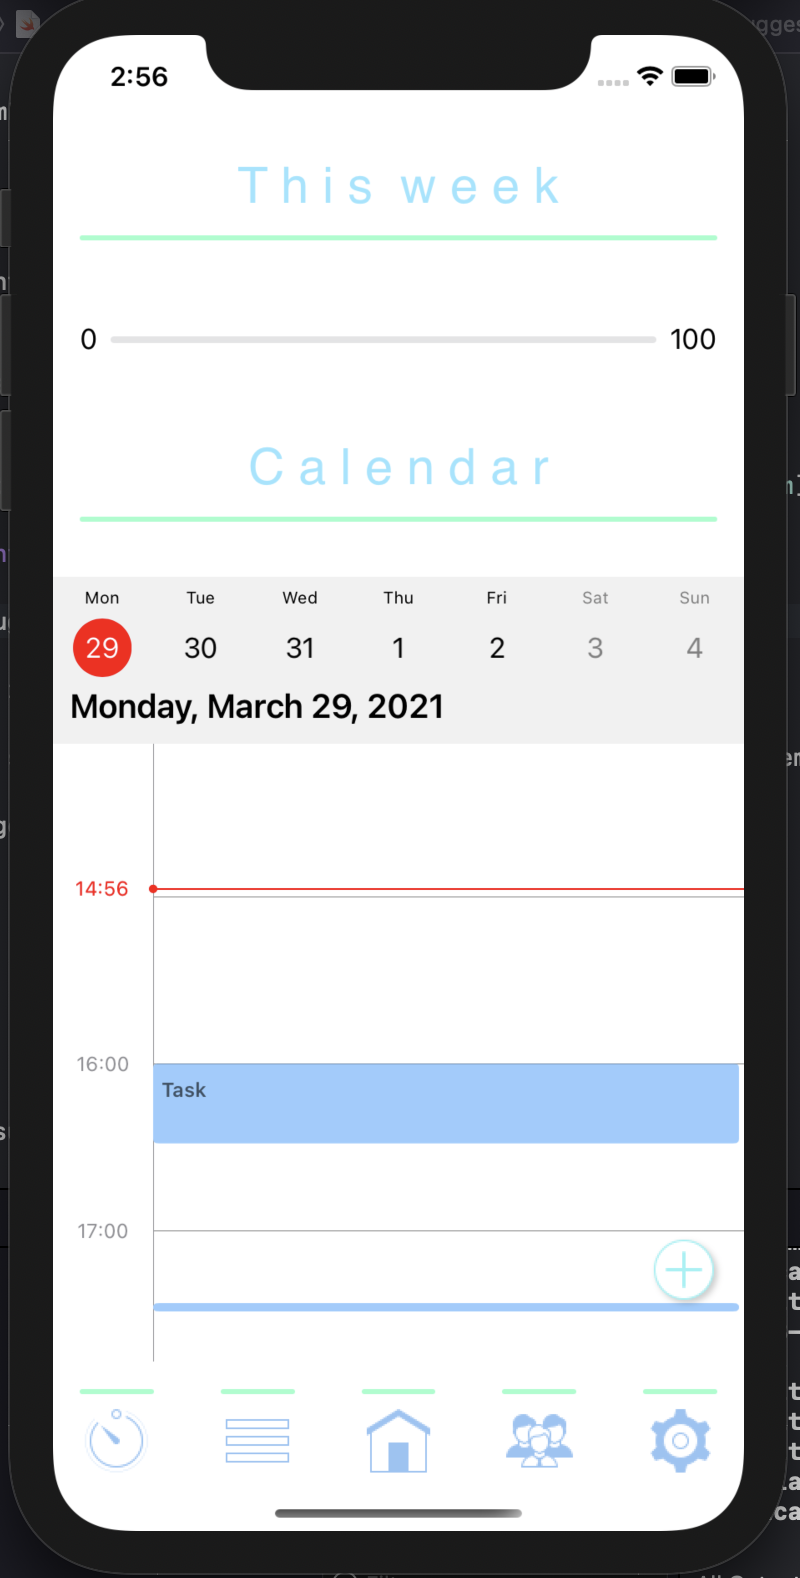
\includegraphics[width=\textwidth]{./graphics/Implementation/Dashboard/calendar this week populated.png}
        \caption{Calendar This Week.}
        \label{fig:cal_this_week_app}
    \end{subfigure}
    \hfill
    \begin{subfigure}[b]{0.3\textwidth}
        \centering
        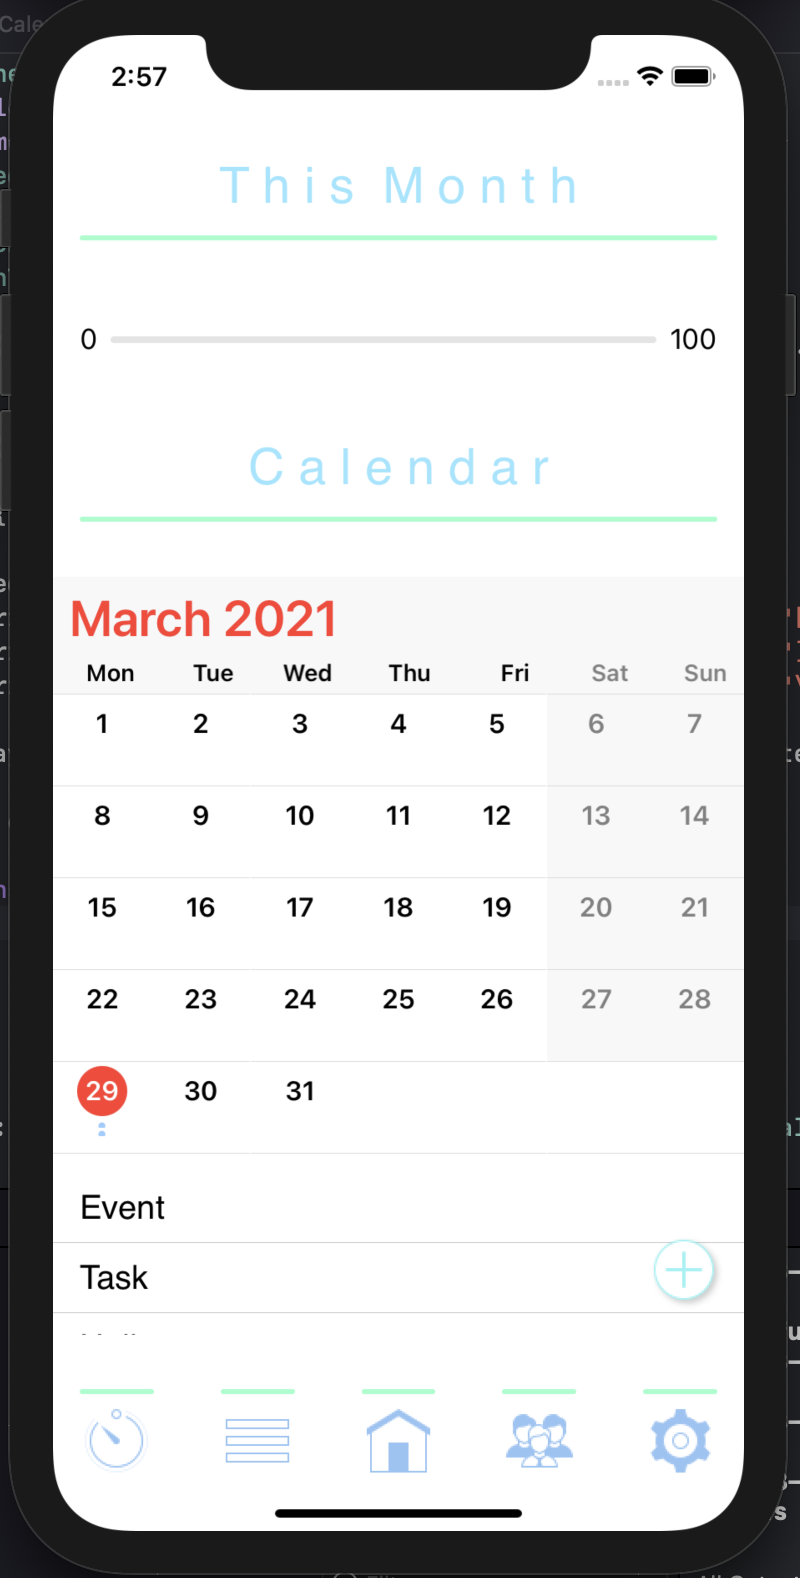
\includegraphics[width=\textwidth]{./graphics/Implementation/Dashboard/calendar this month populated.png}
        \caption{Calendar This Month.}
        \label{fig:cal_this_month_app}
    \end{subfigure}
    \hfill
    \begin{subfigure}[b]{0.3\textwidth}
        \centering
        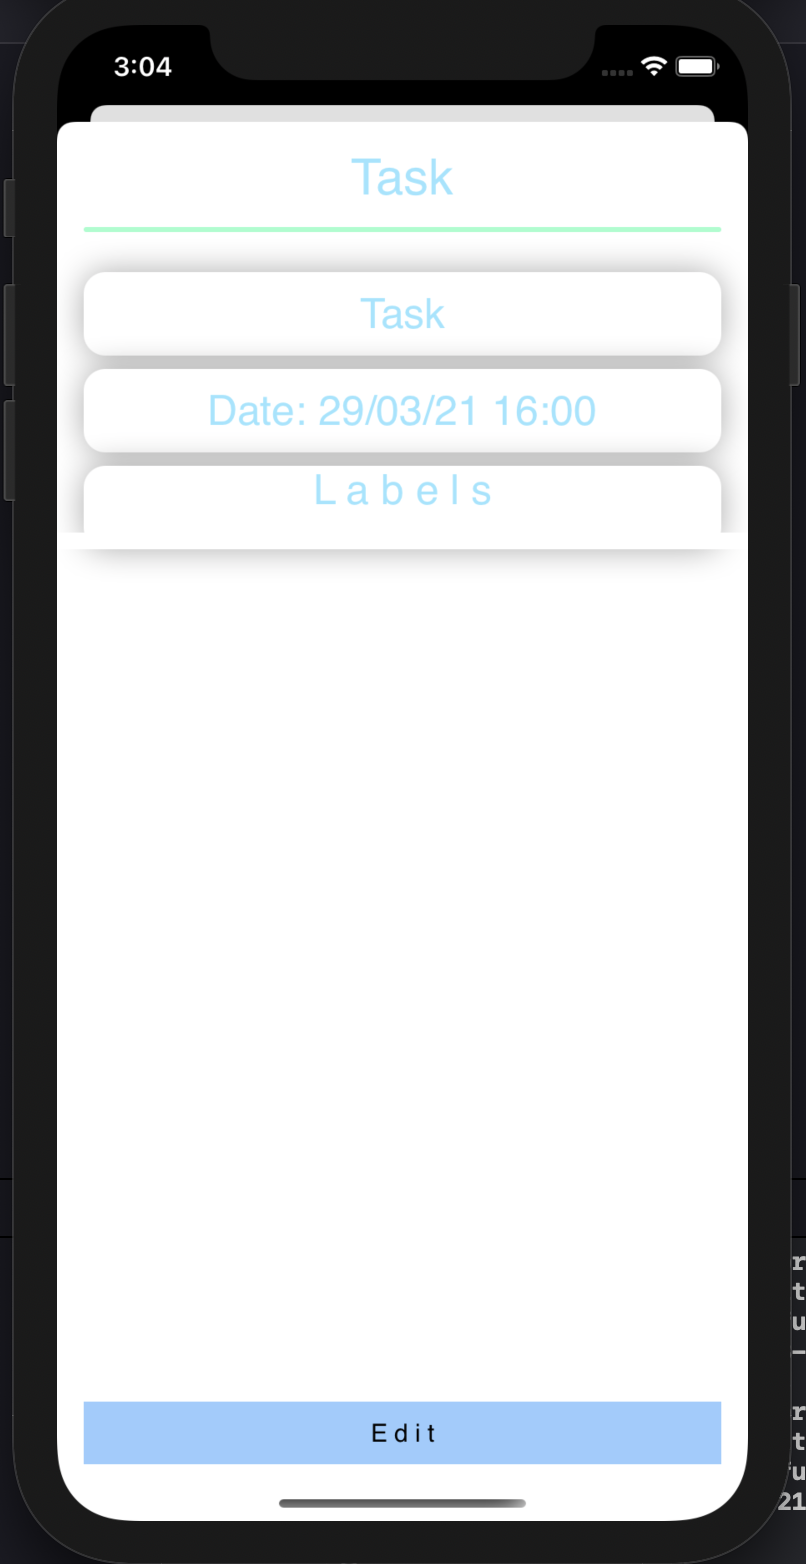
\includegraphics[width=\textwidth]{./graphics/Implementation/Dashboard/task detail.png}
        \caption{Item Detail View.}
        \label{fig:item_detail_app}
    \end{subfigure}
    
    \caption{The calendar views and item detail view.}
    \label{fig:cal_item_app}
\end{figure}
        
        \subsubsection{Back-end}
        \label{subsubsec:dashboard_backend}
        The FirebaseSession class primarily handles the adding and deleting of items and works with Item objects defined within the application to populate the views.  When the dashboard is brought to the foreground, the items stored under the user in the database need to be downloaded to the application. This is done using the retrieveItems function defined in the Firebase Session class.  This function calls the getDocument function in the API and using the document file path, all available items in that path of the database are downloaded.  Each element within the item is converted into the correct object, such as String, Bool, NSDate and added to an array of Item objects, then assigned to the User object to be accessed from within the application.  The function retrieveLabels does a similar task, just in the context of labels instead of items.  Finally, retrieveProgress repeats the task within the context of progress.
        
        When completing an item, the progress counter is incremented by one, and this is then saved to the database using the saveProgress function.  The setData function provided by the Firebase API is called, and this updates the progress value in the database to the correct value.  The boolean tracking whether the item is complete within the Item object is also set to true.  When something is changed in an Item object, the saveItem function is called in Firebase Session. Similarly to updating the progress, it will call the setData API function and update the database with the correct information.  Finally, if the user wishes to delete an item entirely, they can swipe either left or right on that item, which will trigger the deleteItem function.  This calls the document function from the API to locate the relevant item in the database. If this is successfully found, the API's delete function is called, which deletes the item from the database.  The source code snippets for the functions mentioned can be found in the appendix under Section~\ref{app:dashboard_backend}.
        
        \subsection{Add Item}
        \subsubsection{Front-end}
        The add item view is mainly made up of toggle objects within a ScrollView.  The user can type in the name of their desired item in the title text field, which is a custom TextField with a HorizontalLine object as the coloured underline.  The user can then toggle their desired options; if the date or reminder toggle is switched on, a DatePicker object appears in order for a date and time to be chosen, and if the even toggle is switched on, a time interval picker appears to choose the length of time the item will last.  At the bottom of the view, the user can add labels to the item.  When they tap the '+' button, a text field will appear to type the new labels' name, and once they tap the tick button, they can then tap the newly created label, which will be highlighted to show it has been selected.  Once the add button is tapped, the application will return to the dashboard, and the newly added item will be able to be viewed.
        
        Suppose the user decides to set a reminder. In that case, once the add button has been tapped, they will be asked permission by iOS to send them notifications from the application (if this has not already been allowed or disallowed).  Once allow has been tapped, reminders will appear in the devices notification centre at the relevant times.  An example of this can be seen in Figure~\ref{fig:add_item_notifications}.
        
        \begin{figure}[H]
    \centering
    \begin{subfigure}[b]{0.3\textwidth}
        \centering
        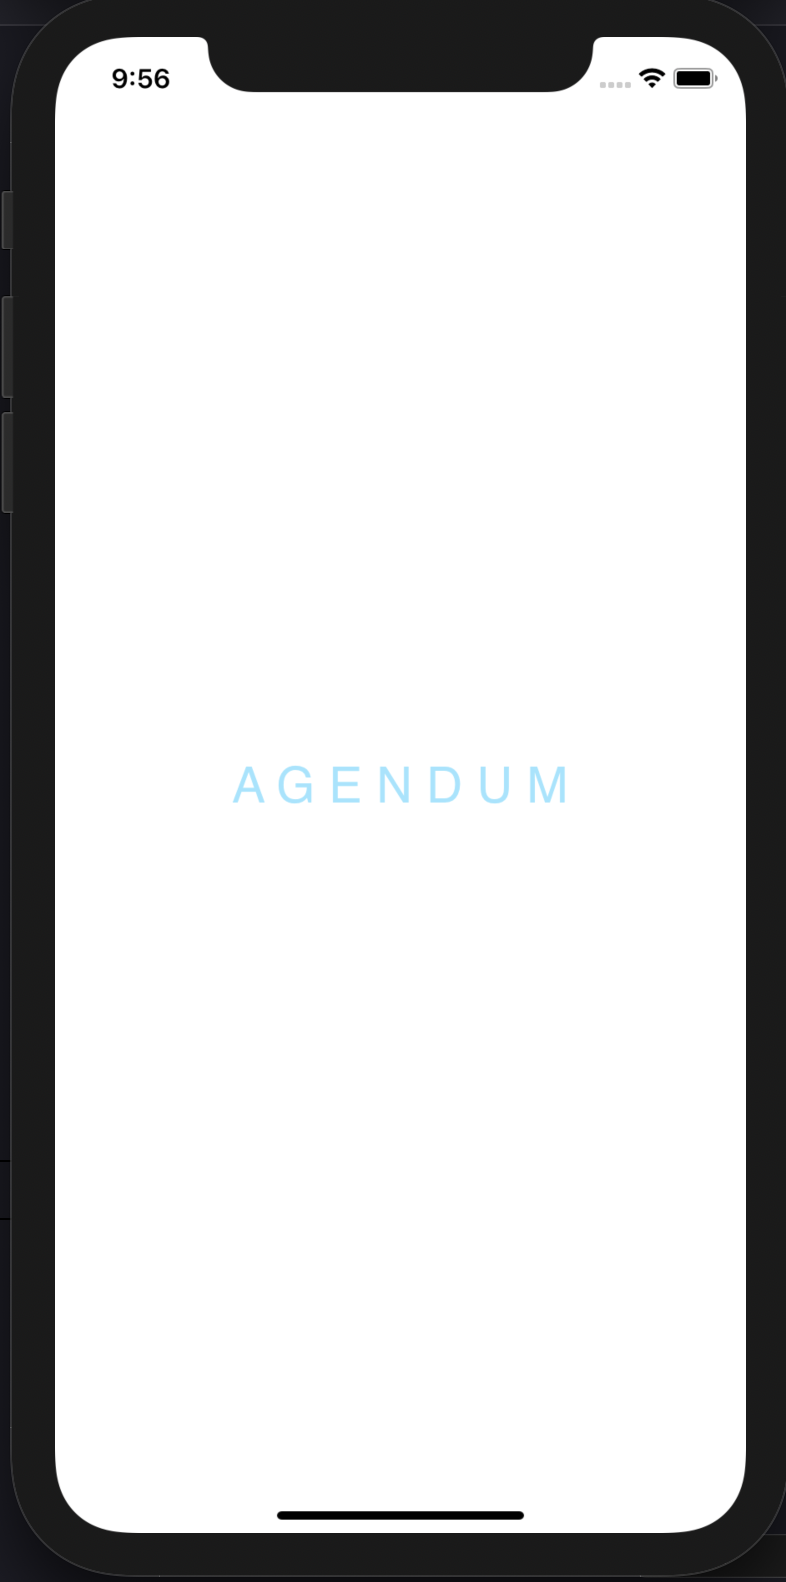
\includegraphics[width=\textwidth]{./graphics/Implementation/Splash_Sign_Up_Sign_In/splash.png}
        \caption{Splash Screen.}
        \label{fig:splash_app}
    \end{subfigure}
    \hfill
    \begin{subfigure}[b]{0.3\textwidth}
        \centering
        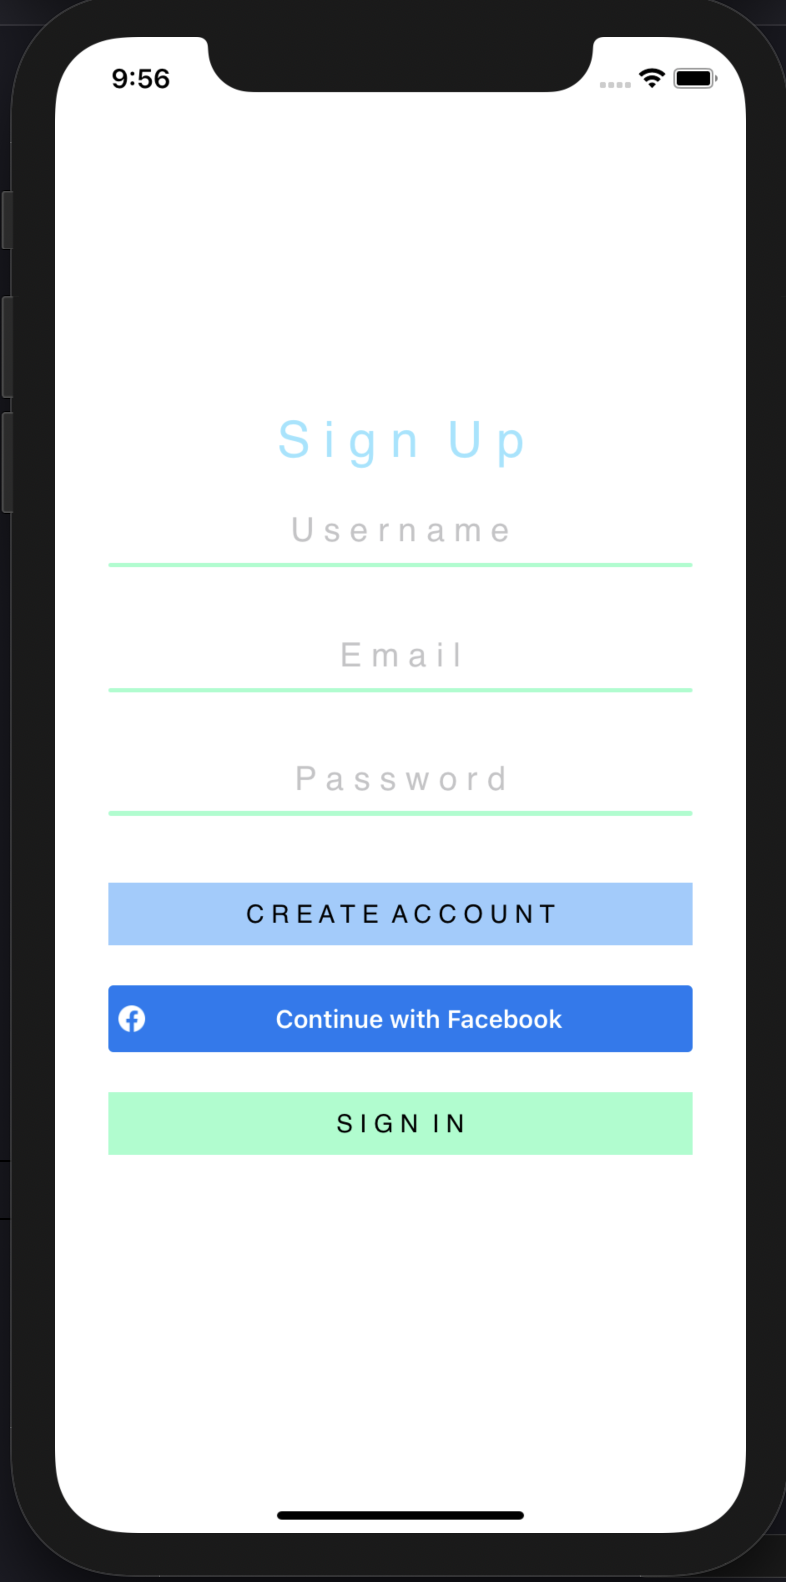
\includegraphics[width=\textwidth]{./graphics/Implementation/Splash_Sign_Up_Sign_In/signup.png}
        \caption{Sign Up.}
        \label{fig:sign_up_app}
    \end{subfigure}
    \hfill
    \begin{subfigure}[b]{0.3\textwidth}
        \centering
        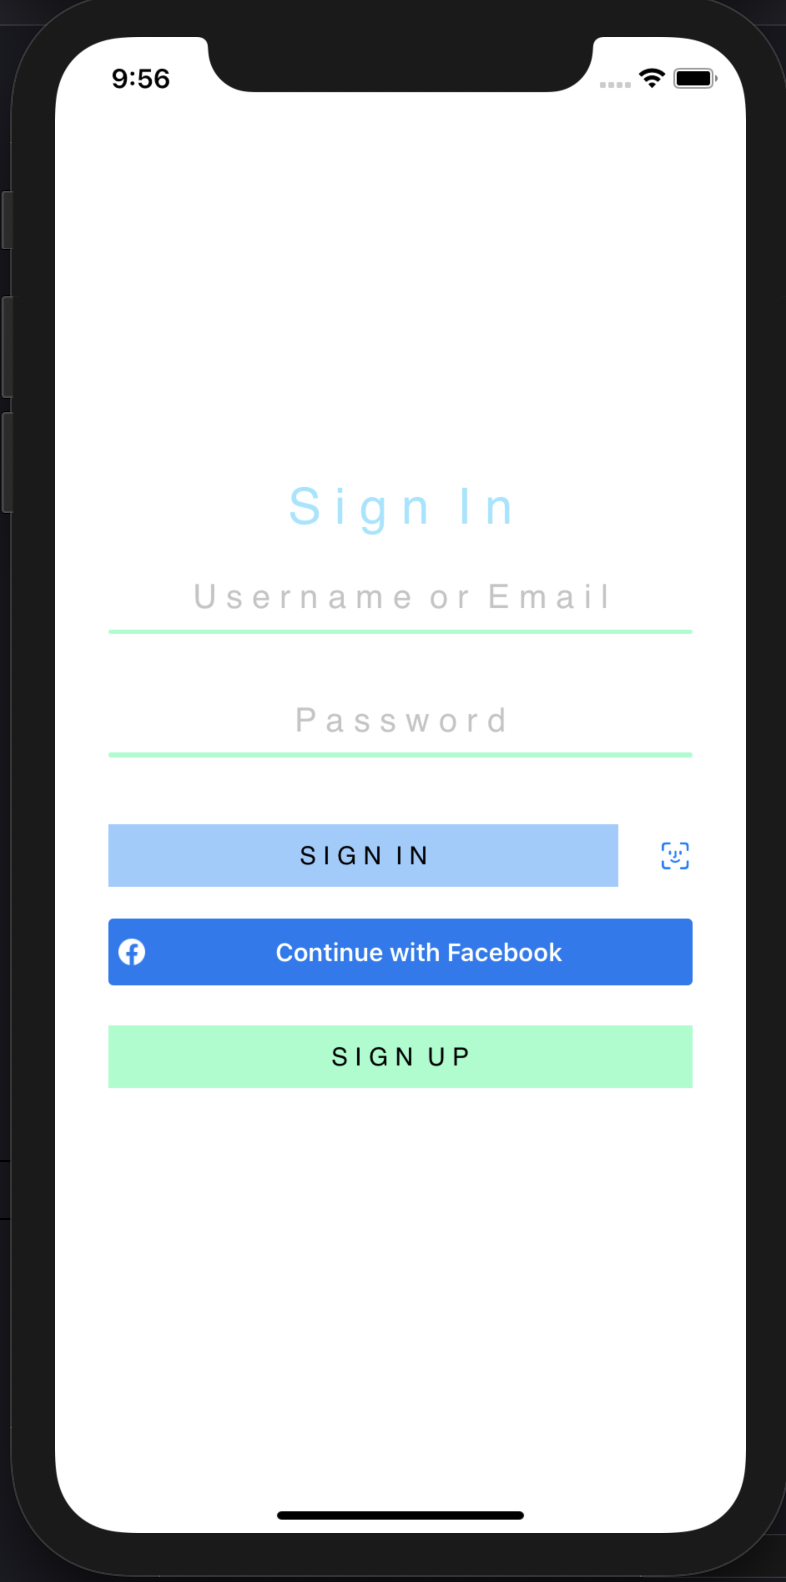
\includegraphics[width=\textwidth]{./graphics/Implementation/Splash_Sign_Up_Sign_In/signin.png}
        \caption{Sign In.}
        \label{fig:sign_in_app}
    \end{subfigure}
    
    \caption{Splash, sign up and sign in views shown in the application.}
    \label{fig:splash_signup_signin_app}
\end{figure}
        
        \subsubsection{Back-end}
        The addItem function defined in the FirebaseSession class handles saving the new item to the database, which is explained in more detail in Section~\ref{subsubsec:dashboard_backend}.
        
        The Notifications class handles the creation of notifications, and an instance of this class is called when the add button is tapped.  The requestPermissions function is called, which generates the alert to allow or deny permissions for notifications to be sent from the application.  If permissions have already been granted, the alert box is not shown.  The generateNotification function then creates the relevant notification by setting a title, and description for the notification and the action, which is performed when the notification is tapped.  It is then added to a notification queue and is released at the desired time.  Apart from what is defined in the application, the notification system is entirely handled by iOS.  The Notifications class code snippets can be seen in Section~\ref{app:add_item_backend} of the appendix.
        
        \subsection{Focus}
        \subsubsection{Front-end}
        The focus view uses the SwiftUIPager framework in order for the user to be able to swipe from the main timer view to the settings.  Within the main view, a custom timer uses the Timer class provided in the Combine framework to countdown from a specified time.  The begin button triggers the countdown and changes to a pause button in order to allow the user to pause the timer.  The break button switches the timer to the desired amount of time the user has set for a break, and the reset button sets the timer back to the original time.  Below these buttons is a text object which shows the item (if one has been selected) that the user has chosen to focus on.
        
        When the user swipes to the left on the timer, they are taken to the settings to set the focus time and the break time.  When either of these items is tapped, a Picker object becomes visible where the user can choose the length of time they wish to set.  Below this, a list of tasks are shown that are yet to be completed; if a user taps on one of these, it will become highlighted, and swiping right on this view will take the user back to the newly set timer.  This functionality can be seen in Figure~\ref{fig:focus_app}.
        
        \begin{figure}[H]
    \centering
    \begin{subfigure}[b]{0.3\textwidth}
        \centering
        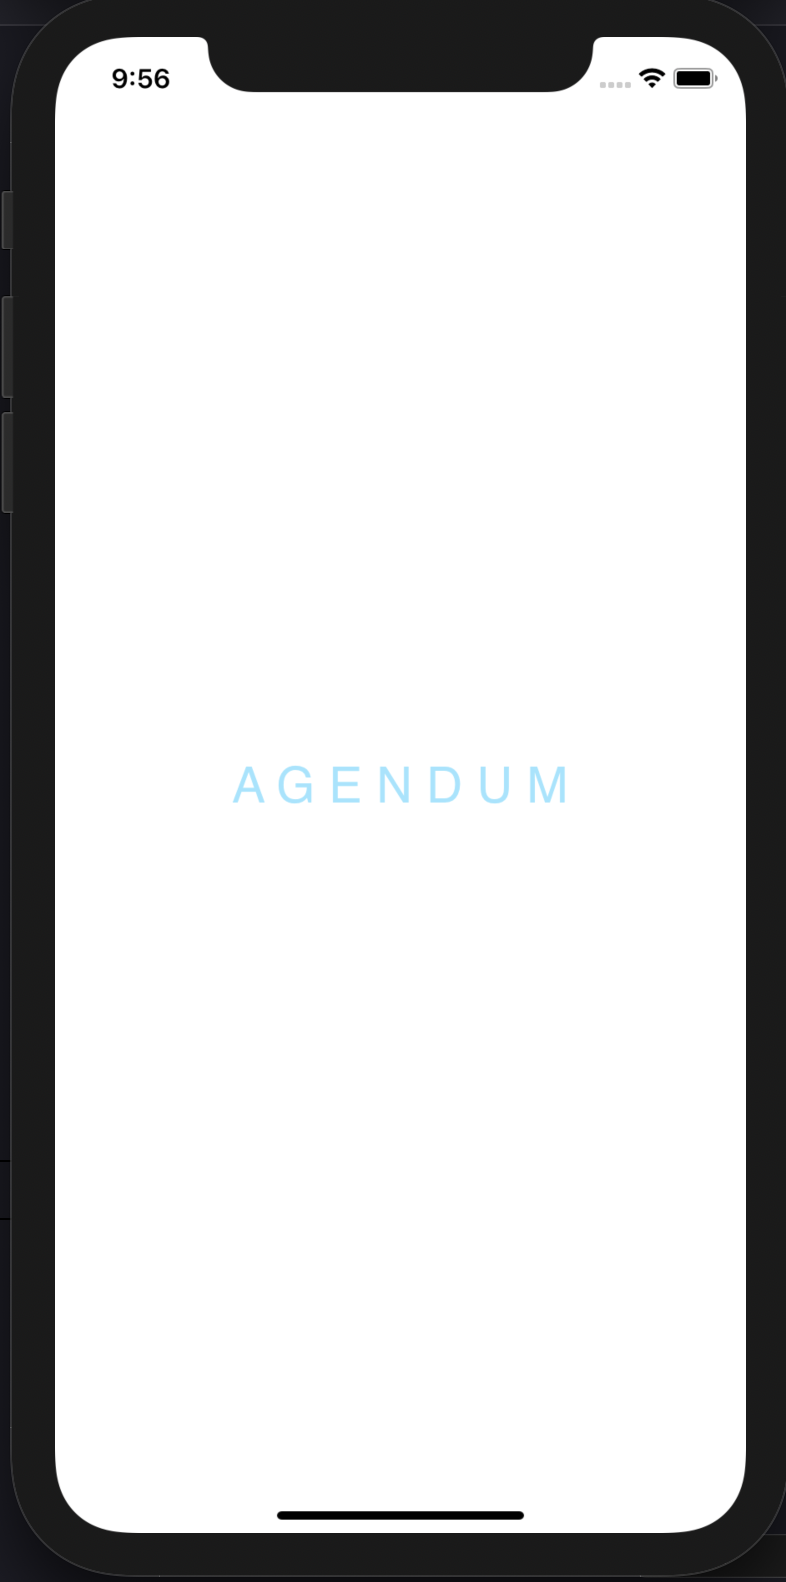
\includegraphics[width=\textwidth]{./graphics/Implementation/Splash_Sign_Up_Sign_In/splash.png}
        \caption{Splash Screen.}
        \label{fig:splash_app}
    \end{subfigure}
    \hfill
    \begin{subfigure}[b]{0.3\textwidth}
        \centering
        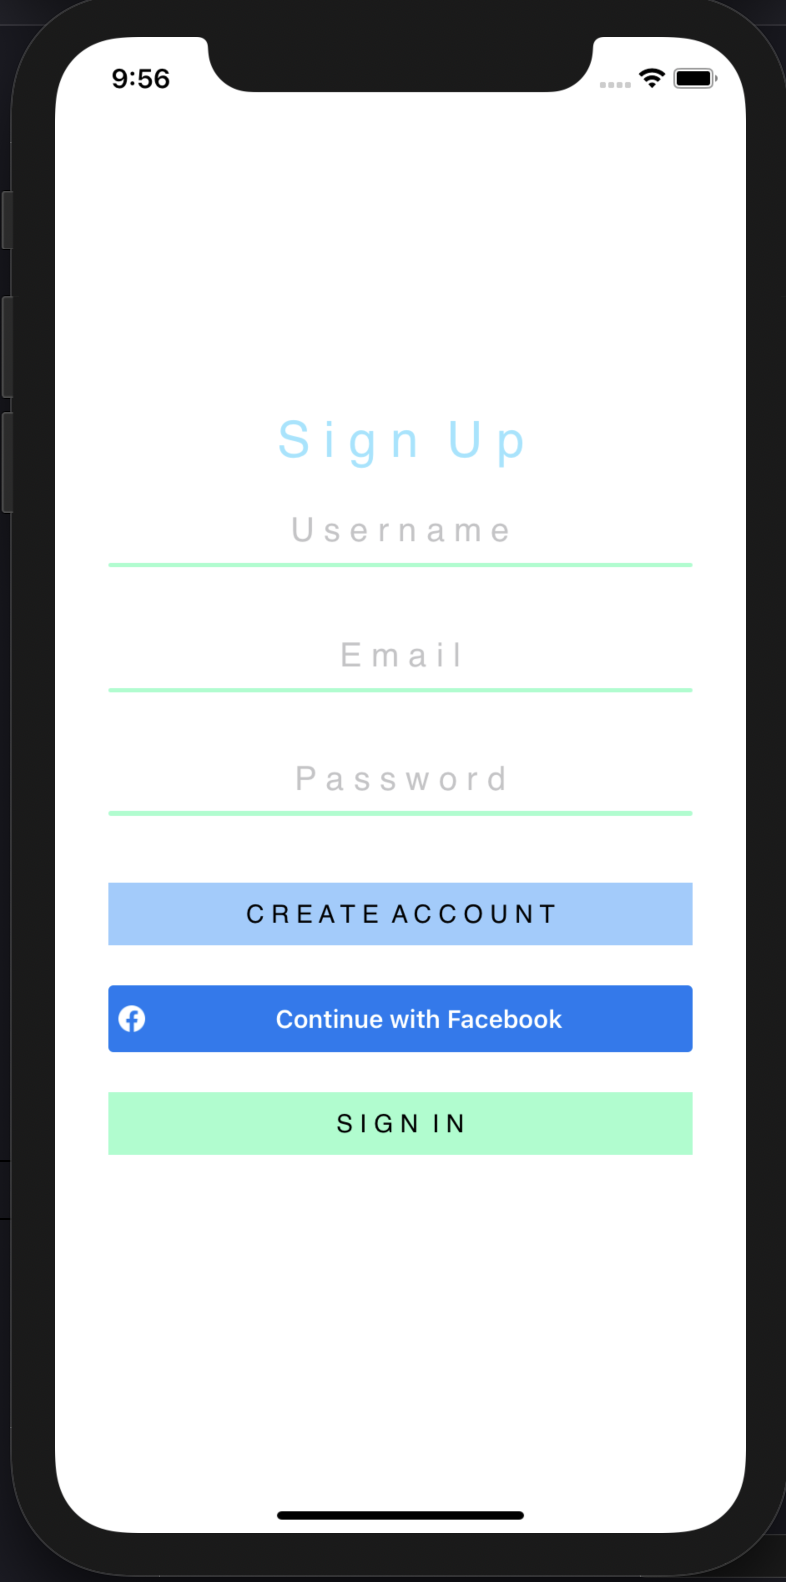
\includegraphics[width=\textwidth]{./graphics/Implementation/Splash_Sign_Up_Sign_In/signup.png}
        \caption{Sign Up.}
        \label{fig:sign_up_app}
    \end{subfigure}
    \hfill
    \begin{subfigure}[b]{0.3\textwidth}
        \centering
        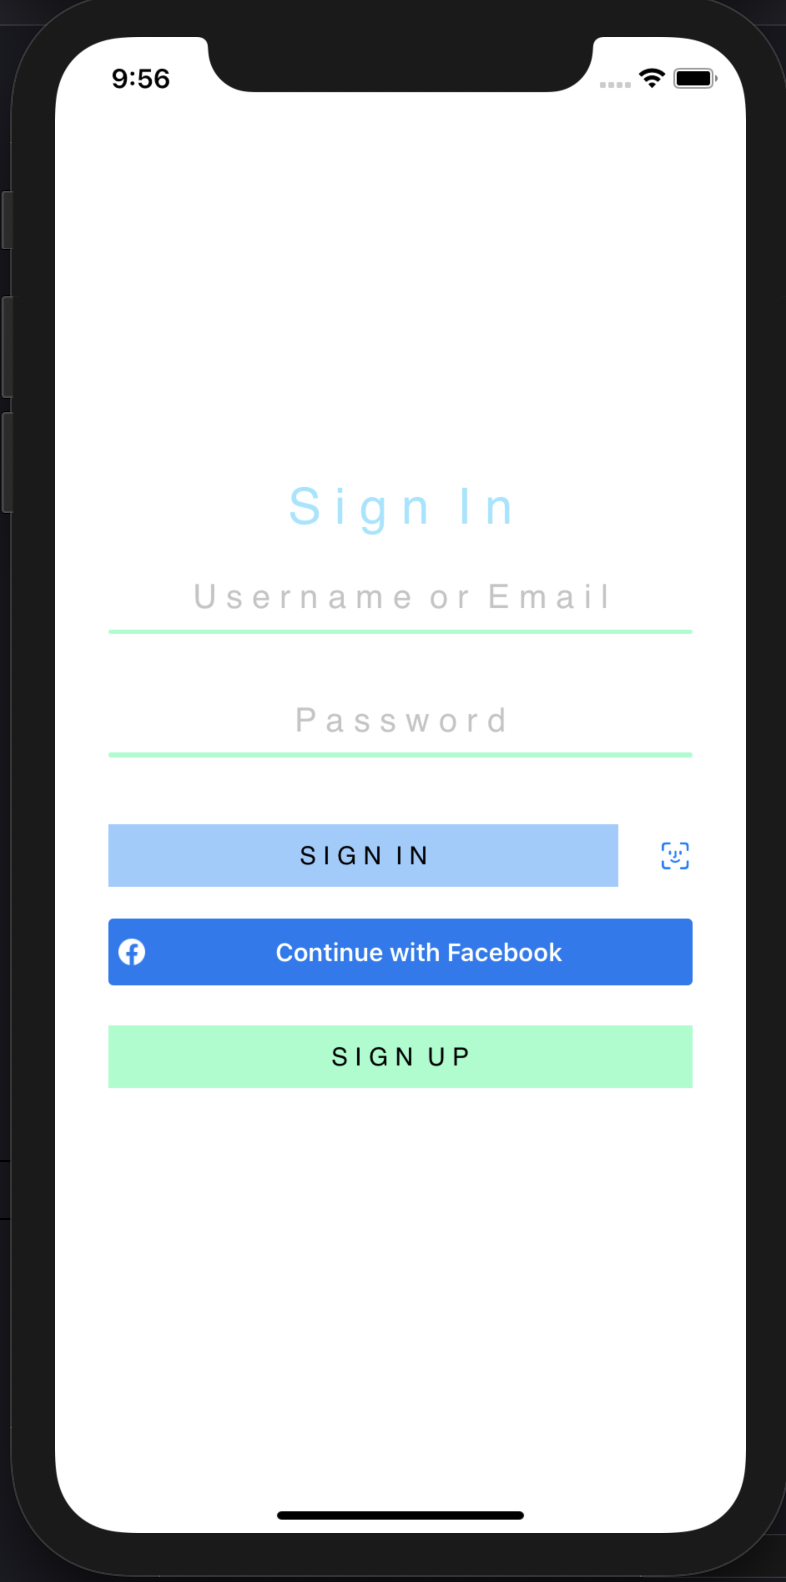
\includegraphics[width=\textwidth]{./graphics/Implementation/Splash_Sign_Up_Sign_In/signin.png}
        \caption{Sign In.}
        \label{fig:sign_in_app}
    \end{subfigure}
    
    \caption{Splash, sign up and sign in views shown in the application.}
    \label{fig:splash_signup_signin_app}
\end{figure}
        
        \subsubsection{Back-end}
        The focus timers' functionality is handled chiefly within the view itself since defining a timer in SwiftUI does not require much computation.  However, to retrieve the tasks in the focus settings, the retrieveItems function is called from the FirebaseSession class.  Details of this function have already been discussed in Section~\ref{subsubsec:dashboard_backend}.
        
        \subsection{All Items}
        \subsubsection{Front-end}
        The All Items view is relatively simple as it is effectively just a list of all the items the user has created.  If an item is not a habit, labelled or has no date set, it will appear in random order at the top of the view.  Items that are due within the next seven days are placed under the 'Due Soon' heading, habits are placed under the 'Habit' heading, items that have been labelled are placed under the title with the name of the label, and items that have been completed are placed under the 'completed' heading.  Tapping the filter button on the left of the search bar will place the items in alphabetical order.  The user can also search for specific items by typing into the search bar.  In Figure~\ref{fig:all_items_app}, an example of this is shown in image C; the user has typed the letter 'E', and items beginning with that letter have been filtered, in this case, an item named 'Event'.
        
        \begin{figure}[H]
    \centering
    \begin{subfigure}[b]{0.3\textwidth}
        \centering
        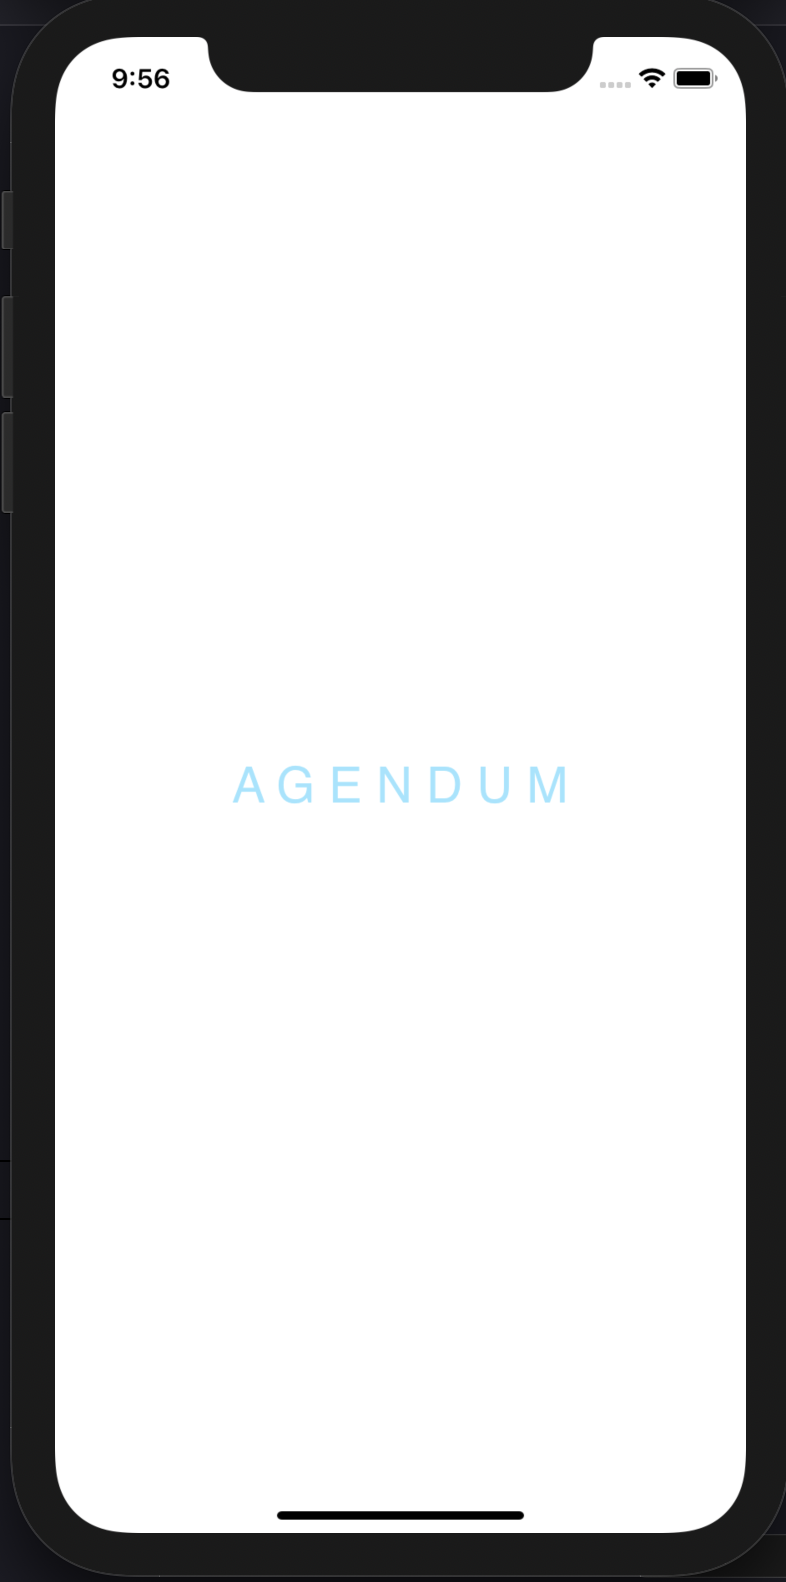
\includegraphics[width=\textwidth]{./graphics/Implementation/Splash_Sign_Up_Sign_In/splash.png}
        \caption{Splash Screen.}
        \label{fig:splash_app}
    \end{subfigure}
    \hfill
    \begin{subfigure}[b]{0.3\textwidth}
        \centering
        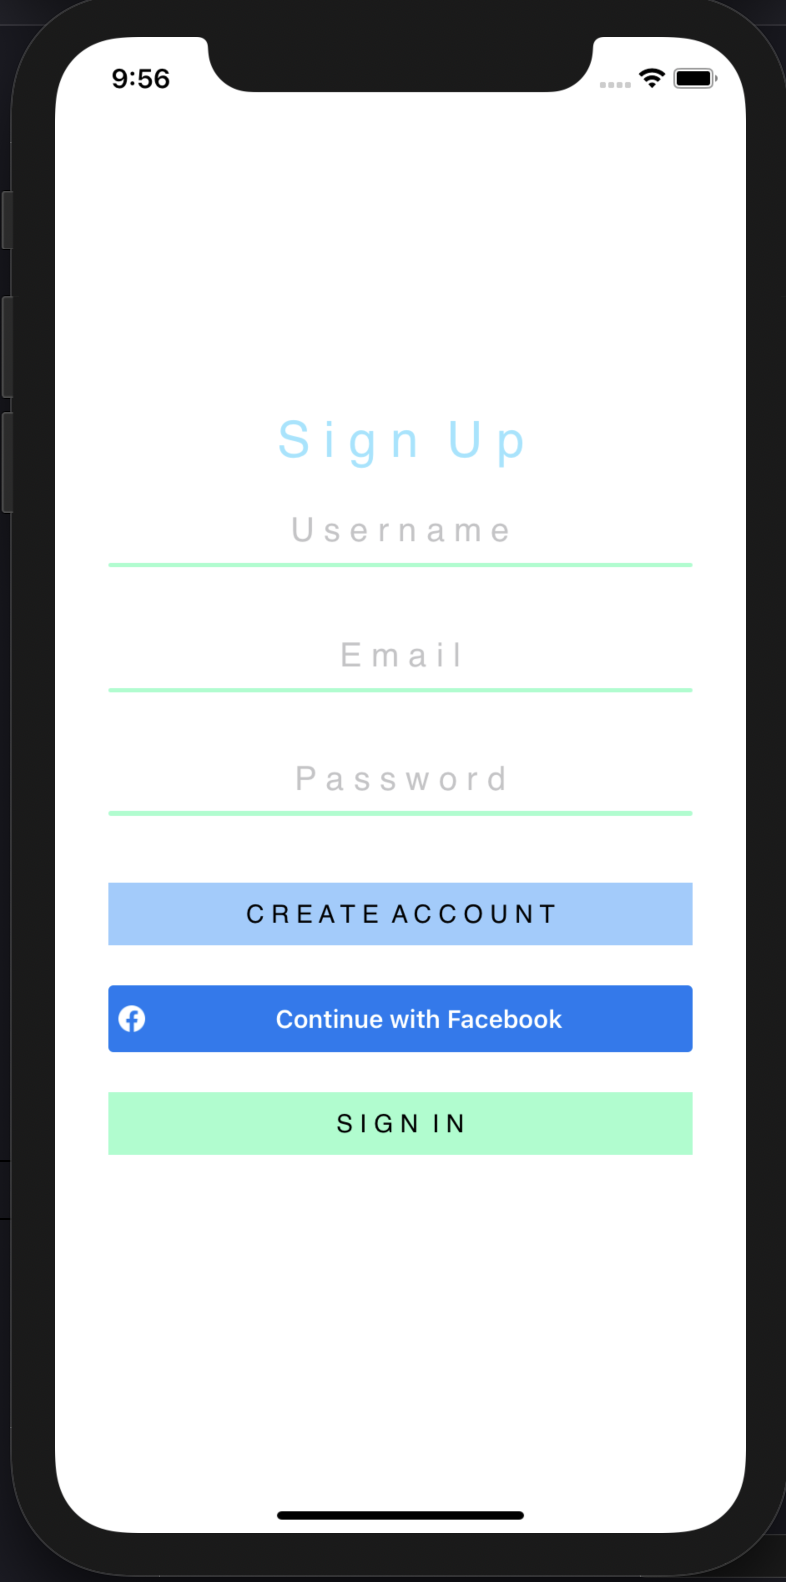
\includegraphics[width=\textwidth]{./graphics/Implementation/Splash_Sign_Up_Sign_In/signup.png}
        \caption{Sign Up.}
        \label{fig:sign_up_app}
    \end{subfigure}
    \hfill
    \begin{subfigure}[b]{0.3\textwidth}
        \centering
        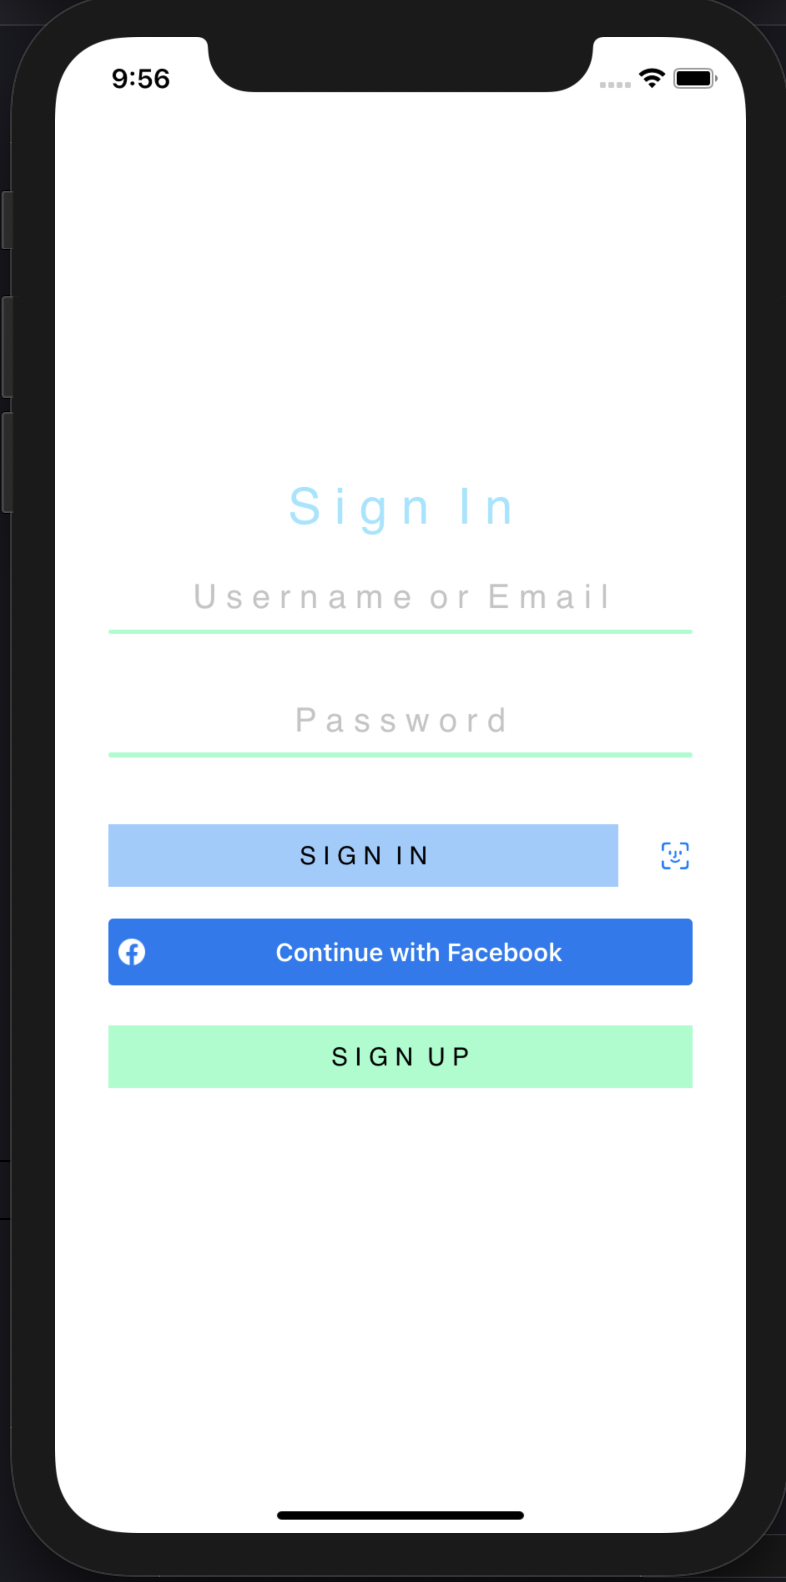
\includegraphics[width=\textwidth]{./graphics/Implementation/Splash_Sign_Up_Sign_In/signin.png}
        \caption{Sign In.}
        \label{fig:sign_in_app}
    \end{subfigure}
    
    \caption{Splash, sign up and sign in views shown in the application.}
    \label{fig:splash_signup_signin_app}
\end{figure}
        
        The view also contains an add button, which will take the user to the add item view.
        
        \subsubsection{Back-end}
        The retrieveItems function defined in the FirebaseSession class is used to download a list of Item objects, which are then parsed to display the items in the view.  The filtering and searching of items are handled in the view source files since they do not require much computation.  Both of them loop through the list of items and extract the relevant items depending on the search/filtering criteria.
        
        \subsection{Friends}
        \subsubsection{Front-end}
        The 'friends' view contains a list of users that the current user has added.  The users' email alongside their current progress points are shown, and at the bottom of the view is the logged in users' progress points.  When the user taps the add button they are taken to the add friend view, where there is a text field to input the user email they wish to add.  Once the user taps the submit button, they are taken back to the main 'friends' view; if the user they added was found it will be shown in their list of friends.  The user can also tap on a friend to be taken to the 'friends detail' view, which shows the friends' progress points and a delete button at the bottom of the view.  If the user taps the delete button, the friend will be removed from their friends list.
        
        \begin{figure}[H]
    \centering
    \begin{subfigure}[b]{0.3\textwidth}
        \centering
        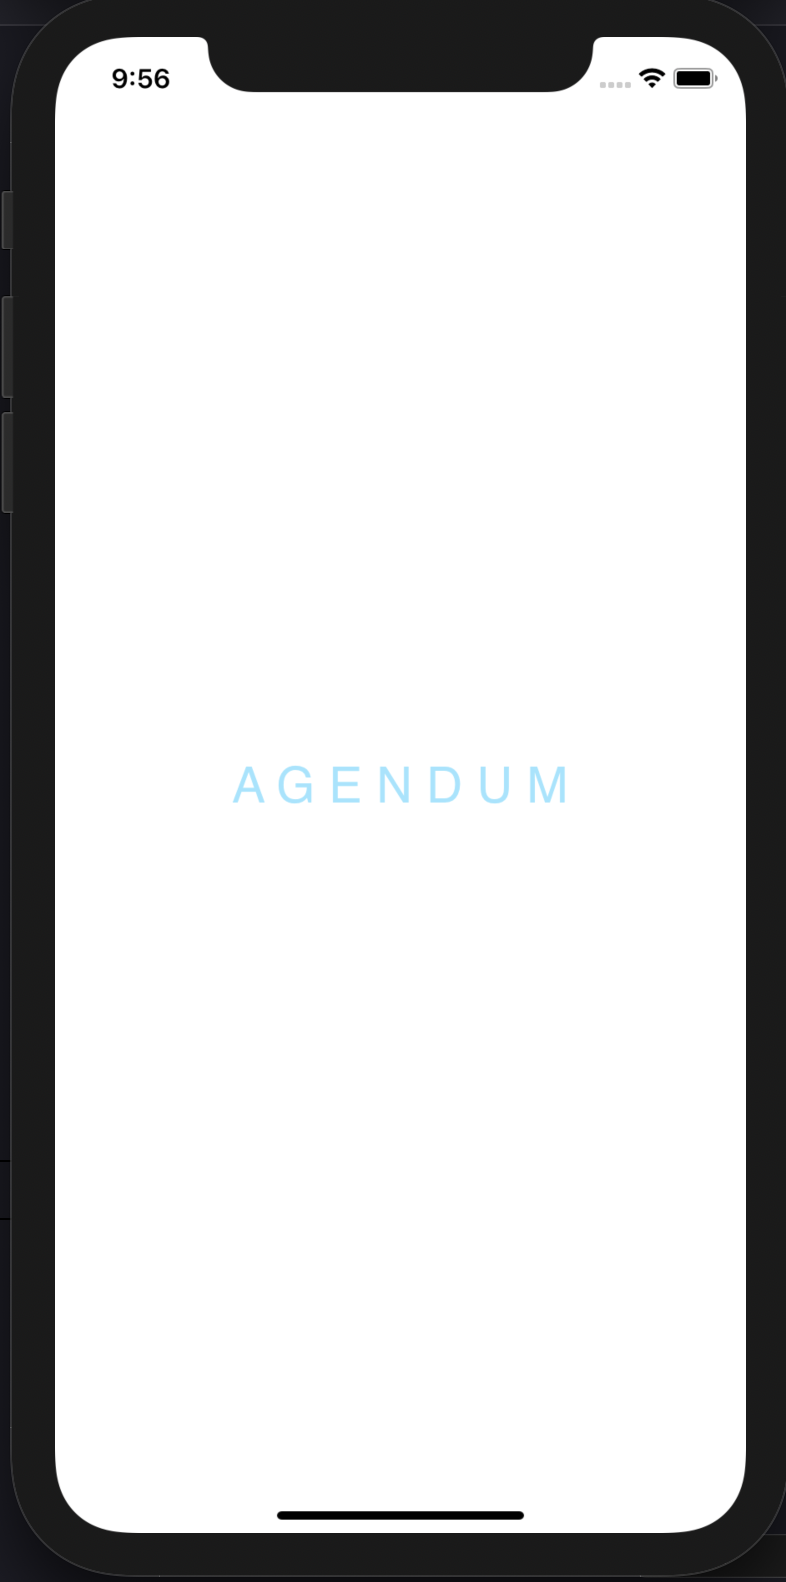
\includegraphics[width=\textwidth]{./graphics/Implementation/Splash_Sign_Up_Sign_In/splash.png}
        \caption{Splash Screen.}
        \label{fig:splash_app}
    \end{subfigure}
    \hfill
    \begin{subfigure}[b]{0.3\textwidth}
        \centering
        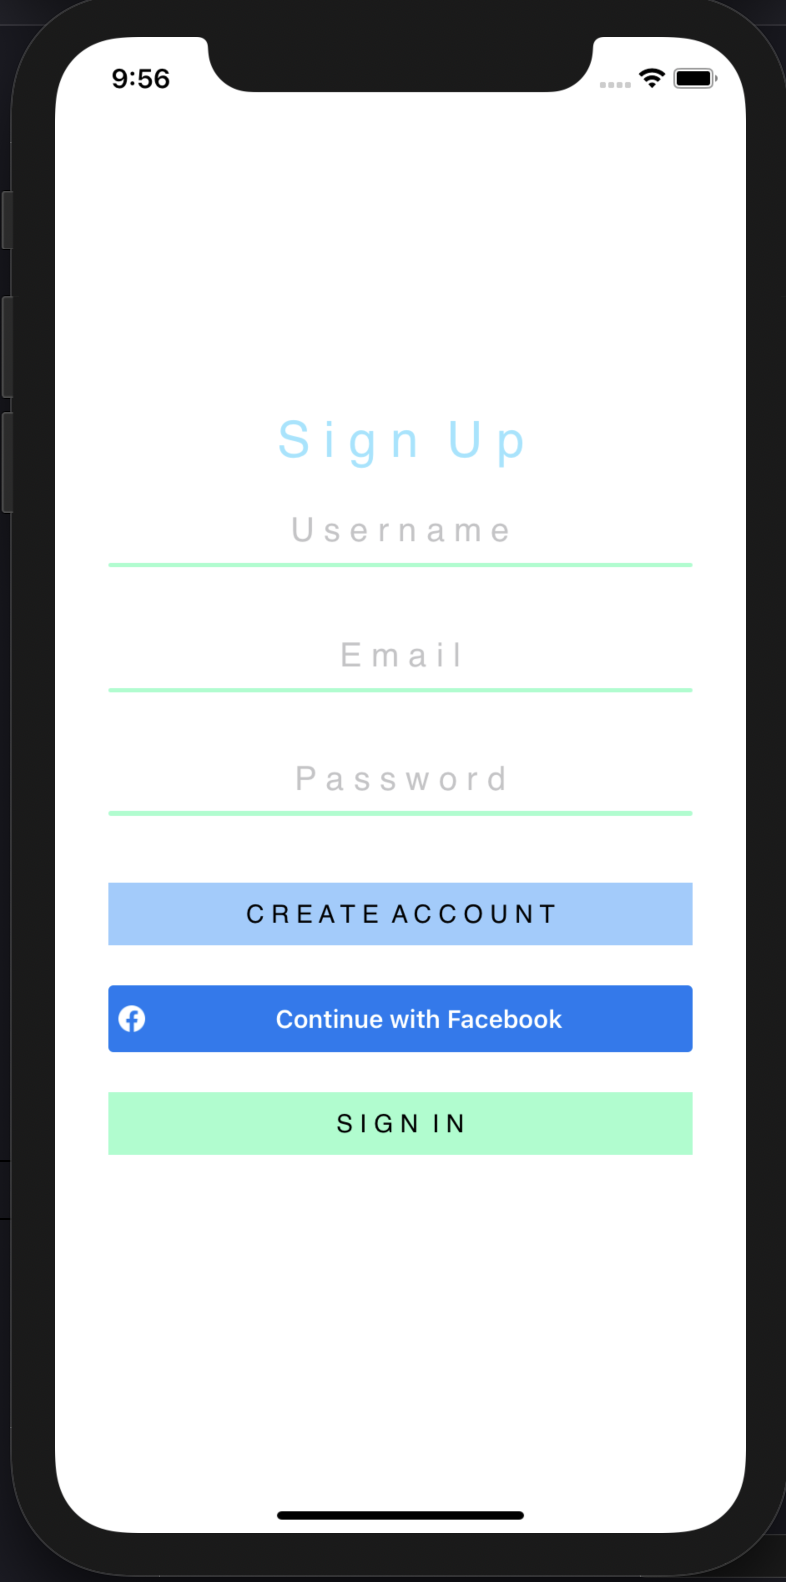
\includegraphics[width=\textwidth]{./graphics/Implementation/Splash_Sign_Up_Sign_In/signup.png}
        \caption{Sign Up.}
        \label{fig:sign_up_app}
    \end{subfigure}
    \hfill
    \begin{subfigure}[b]{0.3\textwidth}
        \centering
        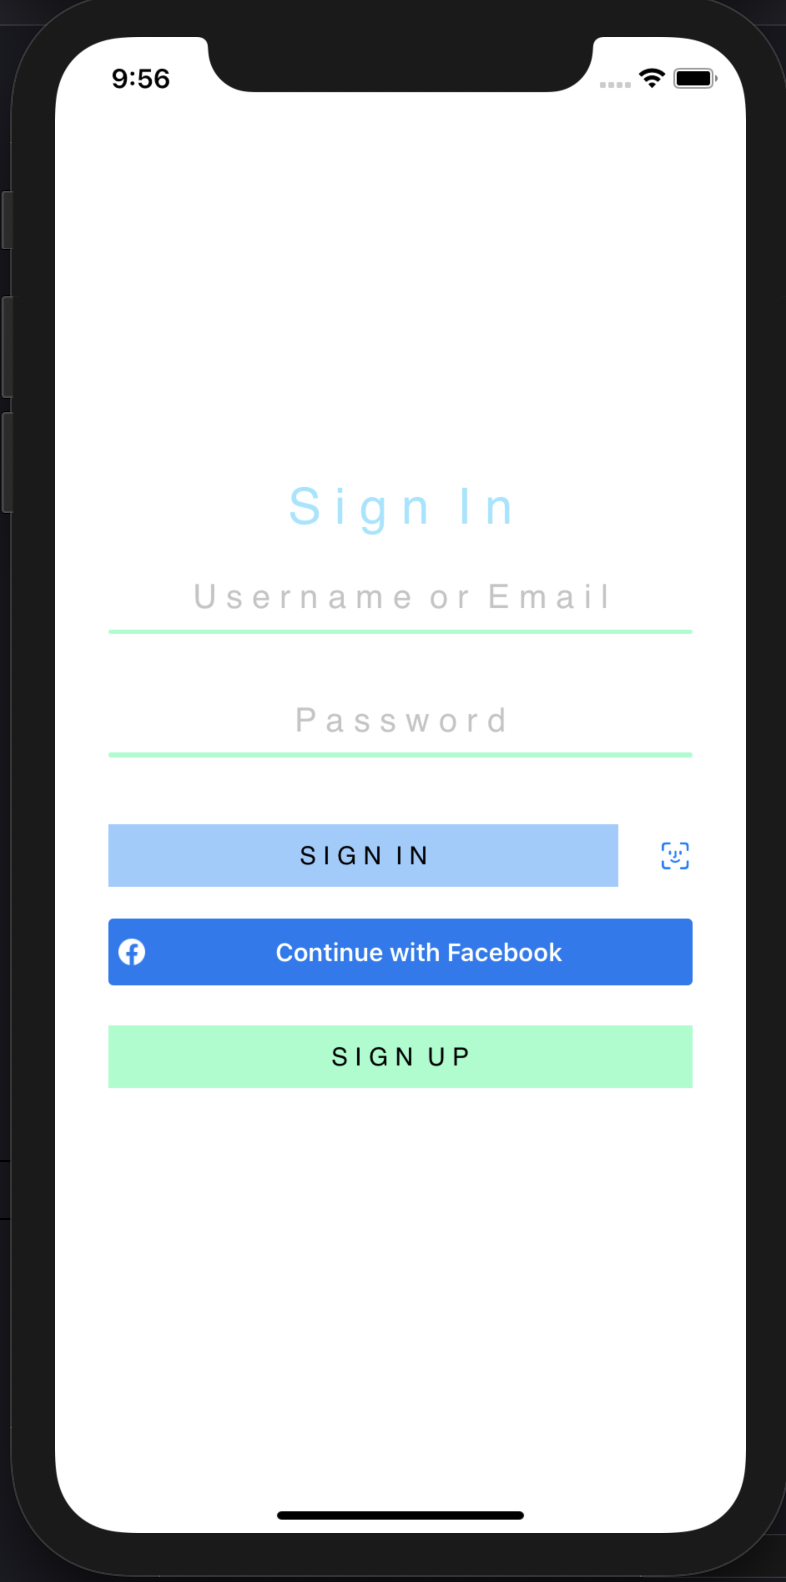
\includegraphics[width=\textwidth]{./graphics/Implementation/Splash_Sign_Up_Sign_In/signin.png}
        \caption{Sign In.}
        \label{fig:sign_in_app}
    \end{subfigure}
    
    \caption{Splash, sign up and sign in views shown in the application.}
    \label{fig:splash_signup_signin_app}
\end{figure}
        
        \subsubsection{Back-end}
        In order to add friends, the findUser function was added to the FirebaseSession class. The findUser function would use the getDocument API call to get a list of available users in the database.  The getDocuments API call would then be made to get the progress and user ID value stored under the user email to be found.  Once this is successful, the followUser function that is also stored in the FirebaseSession class is called.  The followUser function uses the setData API call to add the found user to the logged in users' database so that this information can be downloaded and displayed in the 'friends' view.
        
        If the user wishes to delete a friend, the unfollowUser function is called from the FirebaseSession class.  This function is almost identical to the findUser function, except once the getDocuments call is successful, the data is deleted from the current users' database rather than added.  The code snippets for these functions can be found in Section~\ref{app:friends_backend} of the appendix.
        
        \subsection{Settings}
        \subsubsection{Front-end}
        The settings view is contained of primarily buttons.  From the settings, the user can change their email and password and connect the iOS calendar, log out, delete their account, and activate bio-metric authentication.  When a user taps on either the change email or change password button, they will be asked to re-authenticate as this is a requirement of changing sensitive data in the Firebase database.  Therefore a pop-up will appear to allow the user to enter their password (or the bio-metric pop-up will appear if bio-metrics is enabled).  Once the user is authenticated, a pop-up will appear to change the email or password depending on which button was tapped.
        
        \begin{figure}[H]
    \centering
    \begin{subfigure}[b]{0.3\textwidth}
        \centering
        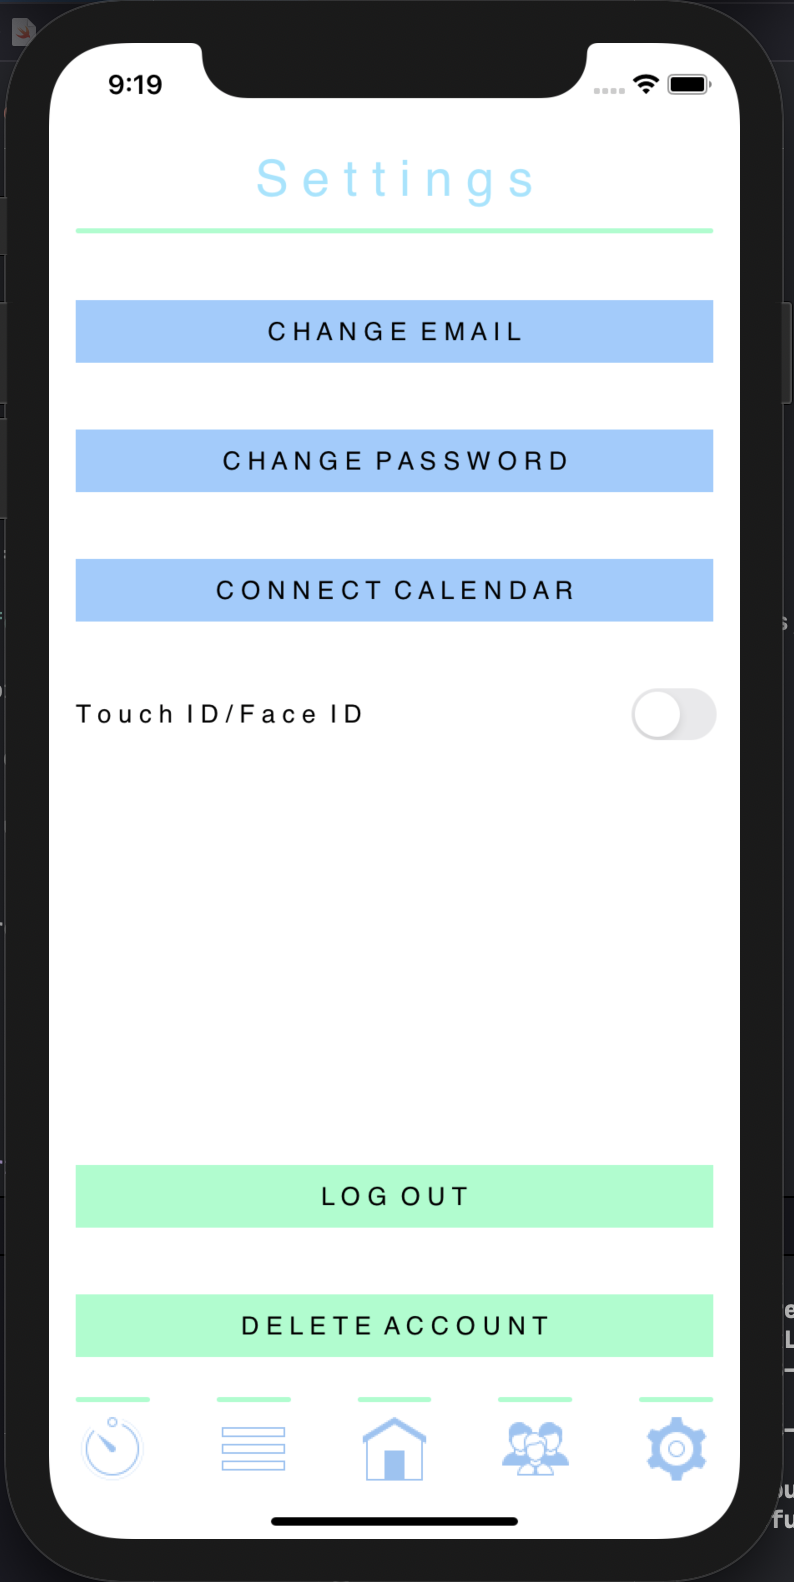
\includegraphics[width=\textwidth]{./graphics/Implementation/Settings/settings.png}
        \caption{Settings View.}
        \label{fig:settings_app}
    \end{subfigure}
    \hfill
    \begin{subfigure}[b]{0.3\textwidth}
        \centering
        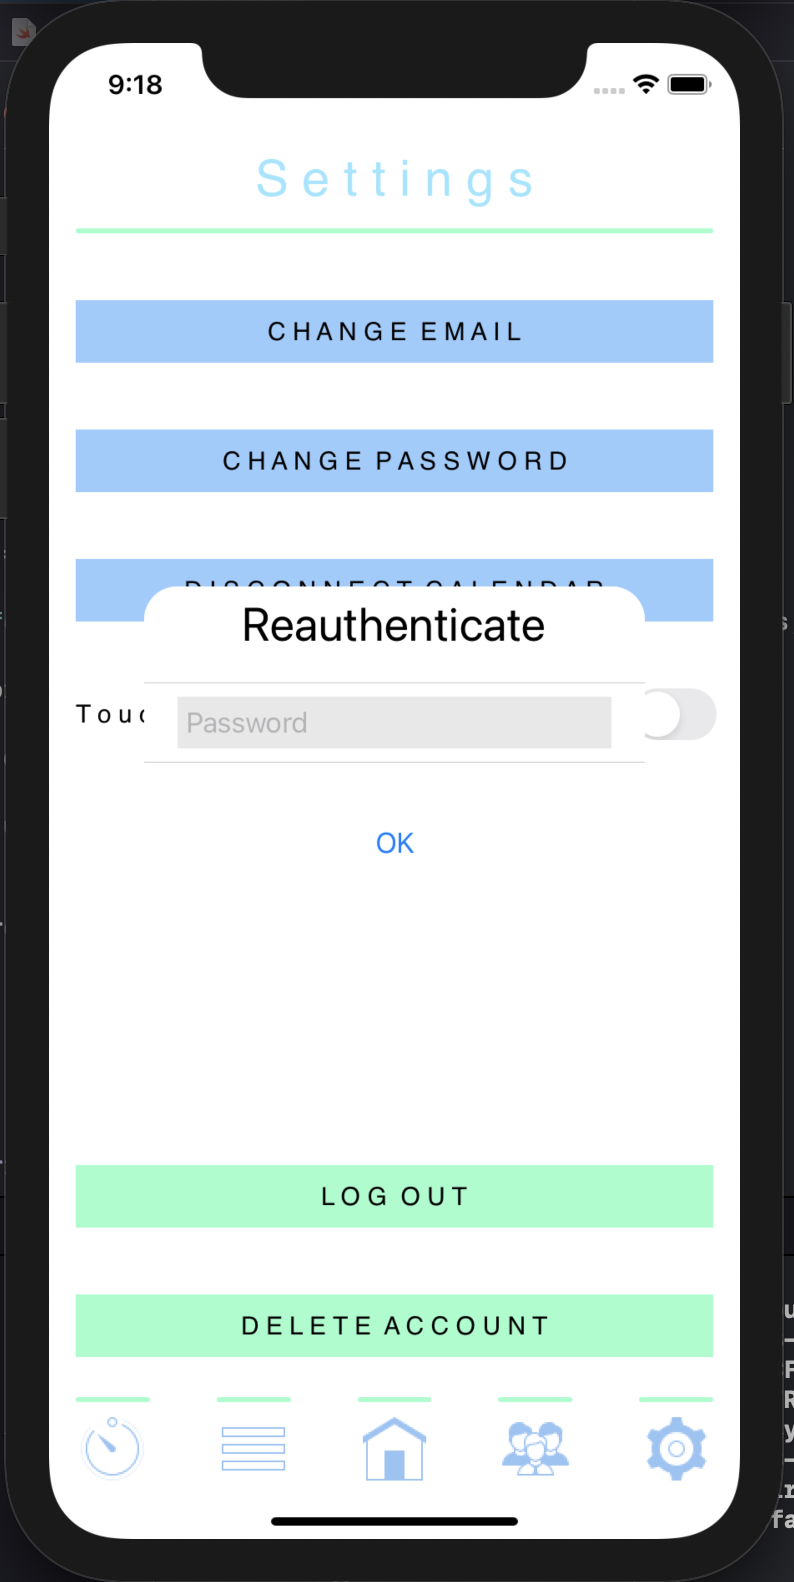
\includegraphics[width=\textwidth]{./graphics/Implementation/Settings/reauth.png}
        \caption{Re-authenticate pop-up.}
        \label{fig:reauth_app}
    \end{subfigure}
    \hfill
    \begin{subfigure}[b]{0.3\textwidth}
        \centering
        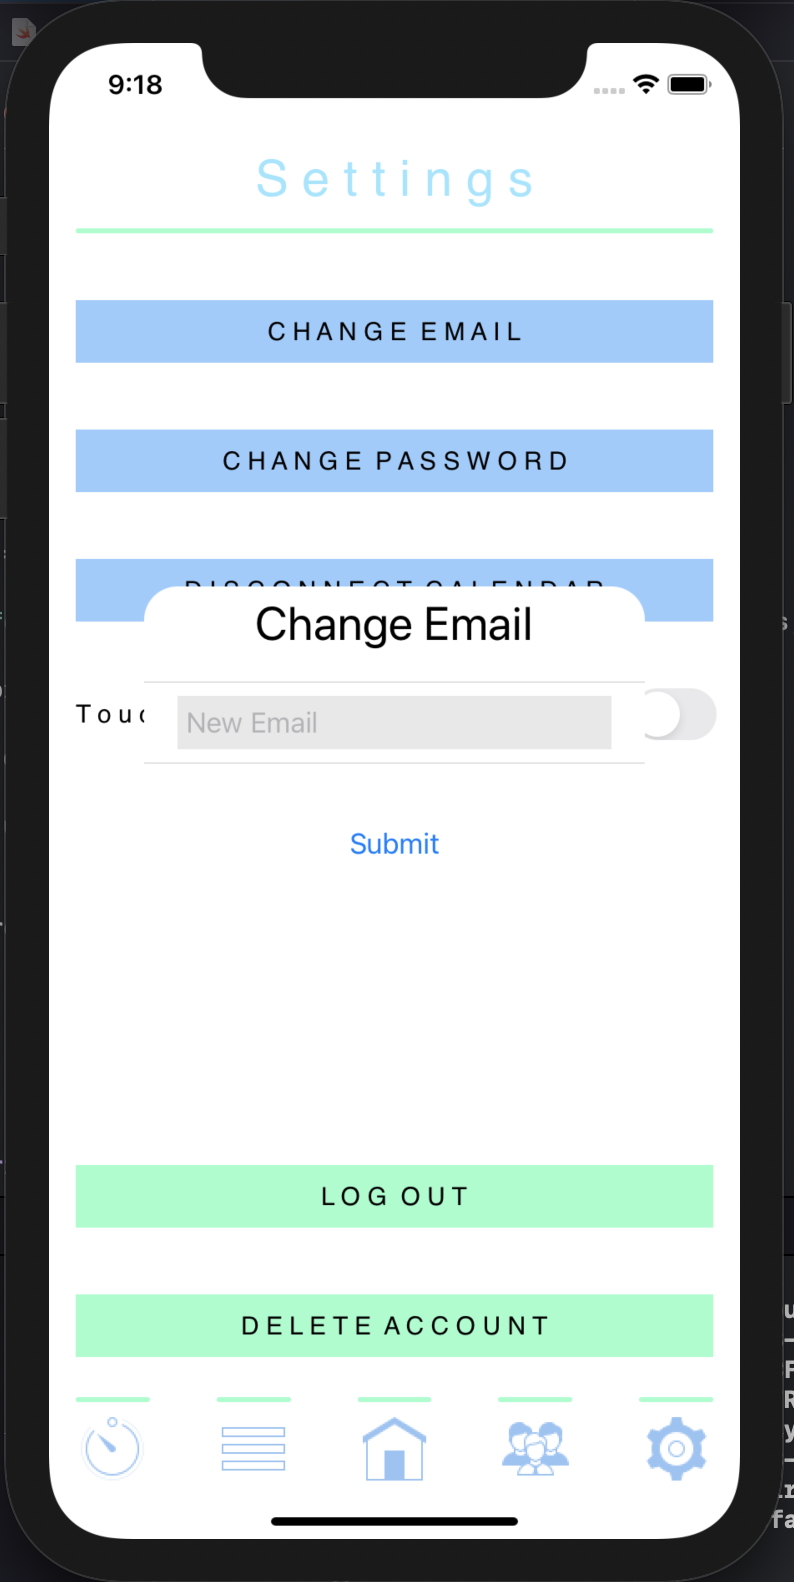
\includegraphics[width=\textwidth]{./graphics/Implementation/Settings/change email.png}
        \caption{Change Email pop-up.}
        \label{fig:change_email_app}
    \end{subfigure}
    
    \caption{Settings View, Re-authenticate and Change Email pop-ups.}
    \label{fig:settings_reauth_change_email}
\end{figure}
        
        Suppose the user toggles the Touch ID/Face ID toggle. In that case, they will be asked to authenticate using the method of biometric authentication on the device (the device used in the project had face ID authentication).  The password pop-up and bio-metric authentication can be found in Section~\ref{app:settings_frontend} of the appendix.  The user can tap the log out button to be taken to the sign-in view or tap the delete button, which will once again cause the application to ask for re-authentication, and once successful; it takes the user to the sign-in screen.
        
        \subsubsection{Back-end}
        To handle the biometric authentication, the Biometrics class was created.  The iOS system mainly handles the bio-metrics, but the tryBiometricAuthentication function will first check whether it is possible to try bio-metric authentication and, if so, generate the touch ID/face ID pop-up so that the user can authenticate.  If it fails, iOS will prompt the user to try again, and if successful, the application will return to the settings screen.  The faceIDAvailable function simply checks what iOS version is installed on the device; if it is newer than iOS11 and the required hardware is available, the function will return true.
        
        When the user wants to change their password, it will be changed both in the Firebase database and in the Apple Keychain storage.  When updating the password in Keychain, the updateGenericPasswordFor function will be called in the KeychainWrapper class, which will find where the password is stored and replace it with the new one.  This function is called from the updatePassword function in the FirebaseSession class after the updatePassword API call is successful.
        
        When the user wishes to change their email, the updateEmail function in FirebaseSession will be called. Similarly to updatePassword, the updateEmail API call will be made to the Firebase database.  In both scenarios, the re-authenticate function will be called, which requires an AuthCredential object as a parameter in order to ensure the user is authenticated to perform sensitive operations in the database.  This is done simply by retrieving the email already stored in the user object and then extracting the password that the user had re-input into the password prompt.
        
        When the user wishes to delete their account, the delete function will be called in the FirebaseSession class.  This calls another function named deleteUserData in FirebaseSession, which deletes all documents in the database related to the user profile, including items, progress, friends and labels.  The user is also required to re-authenticate in this scenario.
        
        Finally, when the user wishes to sign out, the signOut function is called in FirebaseSession. This calls the signOut API call, which simply closes the current session with the Firebase database.
        
    \section{Testing}
    \label{sec:deliverables_testing}
    In this section, the completion of the testing phase will be discussed, including any issues that arose and screenshots the completed test results.
    
    \subsection{Ad-hoc testing}
    After completing each task set in the Trello backlog, various tests would be carried out to ensure the new feature would work as expected.  As these tests were carried out without an initial test plan, they also were not recorded.  An example of a test carried out would be when the add item feature was being implemented.  To ensure the feature was behaving as expected, an item would be added, and then Firebase would be checked to ensure that the item was successfully added to the database.  If a feature did not work as expected, the XCode debugger would be used to pinpoint the issue, and then steps could be taken towards mitigating the problem.  This type of testing proved to be very effective during the implementation; however, if testing were left entirely until after the implementation phase, it would be a very ineffective way of testing as it is difficult to track what has already been tested and what still needs to be tested without the creation of test suites or an existing testing plan.
    
    \subsection{UI Testing}
    Even though time constraints dictated that UI testing was not possible for the entire application, some test cases were created for the sign-up and sign-in process.  Figure~\ref{fig:ui_test_results} shows the results of these tests.
    
    \begin{figure}[H]
    \centering
    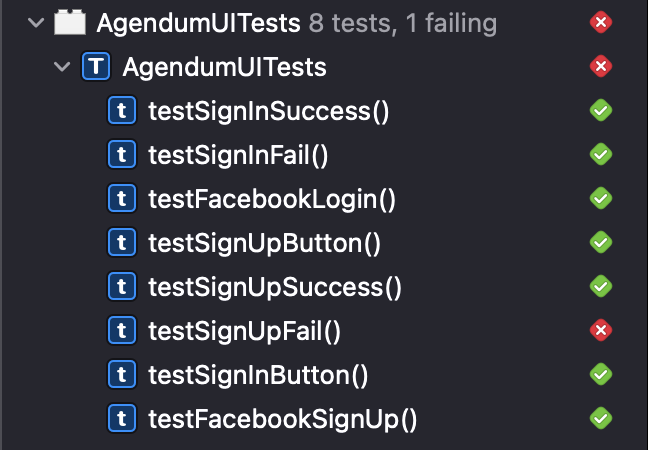
\includegraphics[width=8cm]{./graphics/testing/test results.png}
    \caption{Results from running the UI test suite.}
    \label{fig:ui_test_results}
\end{figure}
    
    As seen from the figure, the testSignUpFail UI test failed, and this is because the create account button cannot be found in the view when the test is running.  This seems to be an error in how the automation was set up rather than an error with the application itself and therefore does not leave a bug that needs to be fixed within the application.  The rest of the tests were successful; the code behind these tests can be found in the appendix under Section~\ref{app:testing_backend}.
    
    \subsection{User testing}
    Unfortunately, due to various complications during the project's implementation, there was no time to send the application out to users to be tested.  However, if this were to go ahead, the application would have been sent to a small group of users with a range of different backgrounds, including students, full-time workers and people of different age groups, to ensure the testing results would be as unbiased as possible at this stage.  A questionnaire would have also been sent out with the application with questions about the application's various features, ease of use, usefulness, and whether any bugs were encountered during the test run.  The questionnaires' results would have then been analysed, and bug fixes and improvements would have been made to the application ready for the second round of user testing.